\documentclass[12pt,a4paper]{report}

% ============================================
% PROFESSIONAL PACKAGES
% ============================================
% Encoding and Fonts
\usepackage[utf8]{inputenc}
\usepackage[T1]{fontenc}
\usepackage{times}
\usepackage{amssymb}  % Provides \checkmark symbol
\usepackage{microtype}  % Professional typography

% Page Layout
\usepackage[left=3cm,right=2.5cm,top=2.5cm,bottom=2.5cm]{geometry}
\usepackage{setspace}

% Headers and Footers
\usepackage{fancyhdr}
\pagestyle{fancy}
\fancyhf{}
\fancyhead[L]{\footnotesize\itshape VocalizeWeb SRS}
\fancyhead[R]{\footnotesize\itshape Namal University}
\fancyfoot[C]{\thepage}
\renewcommand{\headrulewidth}{0.4pt}
\renewcommand{\footrulewidth}{0pt}
\fancypagestyle{plain}{
    \fancyhf{}
    \fancyfoot[C]{\thepage}
    \renewcommand{\headrulewidth}{0pt}
}

% Graphics and Colors
\usepackage{graphicx}
\usepackage{rotating}  % For rotated table headers
\usepackage[dvipsnames,svgnames,table]{xcolor}

% Define Professional Color Scheme
\definecolor{primaryblue}{RGB}{25, 118, 210}
\definecolor{secondaryorange}{RGB}{245, 124, 0}
\definecolor{accentgreen}{RGB}{56, 142, 60}
\definecolor{codebg}{RGB}{248, 249, 250}
\definecolor{lightgray}{RGB}{240, 240, 240}

% Tables
\usepackage{array}
\usepackage{tabularx}
\usepackage{longtable}
\usepackage{booktabs}  % Professional table rules
\usepackage{multirow}
\usepackage{colortbl}

% Hyperlinks and References
\usepackage{hyperref}
\hypersetup{
    colorlinks=true,
    linkcolor=primaryblue,
    filecolor=magenta,      
    urlcolor=primaryblue,
    citecolor=accentgreen,
    pdftitle={VocalizeWeb Software Requirements Specification},
    pdfauthor={Sarmad Sultan, Shehzana Bibi},
    pdfsubject={Voice-to-Voice AI Assistant SRS},
    pdfkeywords={SRS, Voice AI, SaaS, RAG, VocalizeWeb},
    bookmarksnumbered=true,
    bookmarksopen=true,
}
\usepackage[capitalise,noabbrev]{cleveref}  % Smart references

% Title and Section Formatting
\usepackage{titlesec}
\usepackage{tocloft}

\titleformat{\chapter}[display]
{\normalfont\huge\bfseries\color{primaryblue}}{\chaptertitlename\ \thechapter}{20pt}{\Huge}
\titlespacing*{\chapter}{0pt}{-50pt}{40pt}

\titleformat{\section}
{\normalfont\fontsize{14}{17}\bfseries\color{primaryblue}}{\thesection}{1em}{}

\titleformat{\subsection}
{\normalfont\fontsize{12}{14.5}\bfseries}{\thesubsection}{1em}{}

\titleformat{\subsubsection}
{\normalfont\fontsize{12}{14.5}\bfseries\itshape}{\thesubsubsection}{1em}{}

% Code Listings
\usepackage{listings}
\lstdefinestyle{mystyle}{
    backgroundcolor=\color{codebg},
    basicstyle=\ttfamily\small,
    breakatwhitespace=false,
    breaklines=true,
    captionpos=b,
    commentstyle=\color{gray},
    frame=single,
    framerule=0pt,
    framexleftmargin=5pt,
    framexrightmargin=5pt,
    framextopmargin=5pt,
    framexbottommargin=5pt,
    keywordstyle=\color{primaryblue}\bfseries,
    numbers=none,
    showspaces=false,
    showstringspaces=false,
    stringstyle=\color{accentgreen},
    tabsize=2,
    xleftmargin=10pt,
    xrightmargin=10pt,
}
\lstset{style=mystyle}

% Floats and Captions
\usepackage{float}
\usepackage{caption}
\captionsetup{
    font={small},
    labelfont={bf,color=primaryblue},
    labelsep=period,
    justification=centering
}
\captionsetup[table]{position=top,skip=5pt}
\captionsetup[figure]{position=bottom,skip=5pt}

% Boxes and Frames
\usepackage{tcolorbox}
\tcbuselibrary{skins,breakable}

% Info Boxes
\newtcolorbox{infobox}[1][]{
    colback=blue!5,
    colframe=primaryblue,
    fonttitle=\bfseries,
    title=#1,
    sharp corners,
    boxrule=1pt,
    left=5pt,
    right=5pt,
    top=5pt,
    bottom=5pt,
}

\newtcolorbox{warningbox}[1][]{
    colback=orange!5,
    colframe=secondaryorange,
    fonttitle=\bfseries,
    title=#1,
    sharp corners,
    boxrule=1pt,
}

% Lists
\usepackage{enumitem}
\setlist[itemize]{leftmargin=*,itemsep=2pt,parsep=2pt}
\setlist[enumerate]{leftmargin=*,itemsep=2pt,parsep=2pt}

% Line Spacing
\onehalfspacing
\setlength{\parskip}{6pt}

% Justification
\usepackage{ragged2e}
\justifying

% Watermark for Draft (comment out for final)
% \usepackage{draftwatermark}
% \SetWatermarkText{DRAFT}
% \SetWatermarkScale{0.5}
% \SetWatermarkLightness{0.9}

% ============================================
% DOCUMENT BEGINS
% ============================================
\begin{document}

% Cover Page (no headers)
\pagestyle{empty}
% Cover Page - Professional Design (Compact)
\begin{titlepage}
    \centering
    
    % Top decorative line
    \noindent\makebox[\linewidth]{\textcolor{primaryblue}{\rule{\paperwidth}{2pt}}}
    
    \vspace{0.5cm}
    
    % University branding
    {\fontsize{16}{19}\selectfont\textcolor{gray}{NAMAL UNIVERSITY}}\\[0.15cm]
    {\fontsize{12}{14}\selectfont\textcolor{gray}{Department of Computer Science}}
    
    \vspace{0.4cm}
    
    % Document type
    \noindent\fcolorbox{primaryblue}{lightgray}{%
        \parbox{0.6\textwidth}{%
            \centering\vspace{0.15cm}
            {\fontsize{14}{17}\selectfont\bfseries Software Requirements Specification}\\[0.1cm]
            {\fontsize{11}{13}\selectfont IEEE 29148-2018 Compliant}
            \vspace{0.15cm}
        }%
    }
    
    \vspace{0.6cm}
    
    % Project Title
    {\fontsize{32}{38}\selectfont\bfseries\textcolor{primaryblue}{VocalizeWeb}}\\[0.3cm]
    {\fontsize{18}{22}\selectfont\textcolor{gray}{Voice-to-Voice AI Assistant}}\\[0.15cm]
    {\fontsize{14}{17}\selectfont\textit{SaaS Platform for Intelligent Website Integration}}
    
    \vspace{0.6cm}
    
    % Project Logo - Further reduced
    
\includegraphics[width=0.18\textwidth]{logo/image1.png}
    
    \vspace{0.6cm}
    
    % Team information
    {\fontsize{12}{14}\selectfont\bfseries Team Members}\\[0.3cm]
    \begin{tabular}{@{}l@{\hspace{2cm}}r@{}}
        \textbf{Sarmad Sultan} & NUM-BSCS-2022-15 \\[0.1cm]
        \textbf{Shehzana Bibi} & NUM-BSCS-2022-44 \\
    \end{tabular}
    
    \vspace{0.4cm}
    
    % Supervisor
    {\fontsize{12}{14}\selectfont\bfseries Supervisor}\\[0.15cm]
    Ms. Sonia Hassan\\[0.05cm]
    {\small\textit{Lecturer, Department of Computer Science}}
    
    \vfill
    
    % Footer information
    \noindent\makebox[\linewidth]{\textcolor{primaryblue}{\rule{0.8\paperwidth}{0.5pt}}}
    
    \vspace{0.2cm}
    
    {\fontsize{10}{12}\selectfont
    \textbf{Namal University} ~|~ 30-KM, Talagang Road, Mianwali ~|~ \href{https://www.namal.edu.pk}{www.namal.edu.pk}
    }
    
    \vspace{0.2cm}
    
    {\fontsize{14}{17}\selectfont\bfseries January 2026} \hspace{1cm} {\fontsize{10}{12}\selectfont Version 1.0}
    
    \vspace{0.2cm}
    
    % Bottom decorative line
    \noindent\makebox[\linewidth]{\textcolor{primaryblue}{\rule{\paperwidth}{2pt}}}
    
\end{titlepage}
\newpage


% Declaration Page
\pagestyle{plain}
% Declaration Page - Professional Design (Compact)
\chapter*{DECLARATION}
\addcontentsline{toc}{chapter}{Declaration}

\vspace{-0.5cm}

\begin{tcolorbox}[
    colback=white,
    colframe=primaryblue,
    arc=0pt,
    boxrule=1pt,
    left=12pt,
    right=12pt,
    top=10pt,
    bottom=10pt
]

The project report titled \textbf{``VocalizeWeb: Voice-to-Voice AI Assistant''} is submitted in partial fulfillment of the degree of \textbf{Bachelor of Science in Computer Science}, to the Department of Computer Science at Namal University, Mianwali, Pakistan.

\vspace{0.3cm}

We declare that:
\begin{enumerate}[leftmargin=*, itemsep=2pt, parsep=0pt]
    \item This is an original work completed by the undersigned team members under the supervision of \textbf{Ms. Sonia Hassan}.
    \item No part of this project report has been plagiarized, and all external sources have been properly cited following IEEE citation standards.
    \item This work has not been submitted for any other degree or qualification at any other institution.
    \item We have read and understood the university's policies on academic integrity and plagiarism.
\end{enumerate}

\end{tcolorbox}

\vspace{0.5cm}

% Team signatures
\noindent\textbf{\textcolor{primaryblue}{Team Members}}

\vspace{0.3cm}

\begin{table}[H]
\centering
\begin{tabular}{@{}p{5cm}p{4.5cm}p{4cm}@{}}
\textbf{Name} & \textbf{University ID} & \textbf{Signature} \\[0.2cm]
\midrule
Sarmad Sultan & NUM-BSCS-2022-15 & \hrulefill \\[0.4cm]
Shehzana Bibi & NUM-BSCS-2022-44 & \hrulefill \\
\end{tabular}
\end{table}

\vspace{0.5cm}

% Supervisor section
\noindent\textbf{\textcolor{primaryblue}{Supervisor Endorsement}}

\vspace{0.3cm}

\noindent I certify that this project has been completed under my supervision and meets the standards required for submission.

\vspace{0.5cm}

\begin{table}[H]
\centering
\begin{tabular}{@{}p{5cm}p{4.5cm}p{4cm}@{}}
\textbf{Name} & \textbf{Designation} & \textbf{Signature \& Date} \\[0.2cm]
\midrule
Ms. Sonia Hassan & Lecturer, CS Dept. & \hrulefill \\
\end{tabular}
\end{table}

\newpage


% Front Matter with Roman Numerals
\pagenumbering{roman}
\setcounter{page}{1}

% Abstract

\chapter*{Abstract}
\addcontentsline{toc}{chapter}{Abstract}

\vspace{0.3cm}

This Software Requirements Specification (SRS) document describes \textbf{VocalizeWeb}, a comprehensive software platform designed to provide intelligent conversational assistance capabilities for websites. The system is built to enable website owners to deploy AI-powered virtual assistants that can help end users find information quickly and accurately through natural language interactions. These interactions can occur through either text-based chat or voice-based conversations, providing flexibility based on user preferences and accessibility needs.

The platform is specifically intended for two primary user groups. First, website administrators and business owners who wish to improve the user experience on their websites and make their content more accessible to visitors. Second, end users who are visiting these websites and seeking efficient alternatives to manually navigating through menus and pages to find information. VocalizeWeb addresses this need by implementing a retrieval-augmented generation (RAG) system, which means the AI assistant retrieves relevant information from the website's actual content before generating responses, ensuring accuracy and relevance rather than relying on the AI's general knowledge.

The technical scope of this software encompasses several major capabilities. It includes the deployment of conversational interfaces that can be embedded into existing websites, comprehensive content management features that allow website owners to control what information the assistant can access, and a multi-tenant service delivery architecture that allows multiple clients to use the same underlying infrastructure while keeping their data completely isolated. The platform operates as a Software-as-a-Service (SaaS) solution, meaning website owners can integrate it into their existing web properties without needing to host or maintain the underlying infrastructure themselves.

This SRS document specifies the functional and non-functional requirements, system architecture, constraints, and acceptance criteria for VocalizeWeb. It is organized following IEEE 29148-2018 standards and serves as the foundation for system design, development, and validation activities.

\vspace{0.5cm}

\begin{center}
\begin{tabular}{@{}lll@{}}
\toprule
\textbf{Keywords} & & \\
\midrule
Conversational AI & Website Assistant & Voice Interface \\
Multi-Modal Interface & SaaS Platform & RAG Architecture \\
\bottomrule
\end{tabular}
\end{center}

\newpage


% Table of Contents
\pagestyle{fancy}
\tableofcontents
\newpage

% List of Figures
\addcontentsline{toc}{chapter}{List of Figures}
\listoffigures
\newpage

% List of Tables
\addcontentsline{toc}{chapter}{List of Tables}
\listoftables
\newpage

% ============================================
% MAIN CONTENT - Arabic Numerals
% ============================================
\pagenumbering{arabic}
\setcounter{page}{1}

% Chapter 1: Introduction
% Chapter 1: Introduction - Revised for Intelligent Content Management Platform
\chapter{Introduction}

The digital transformation of business operations has created unprecedented demand for intelligent, always-available customer engagement solutions. However, the fundamental challenge extends beyond mere availability---users expect instant, accurate answers without navigating complex website hierarchies or waiting for human agents. VocalizeWeb addresses this need by providing a multi-modal conversational AI platform that enables natural language interaction through both text and voice.

This document specifies the requirements for VocalizeWeb, an intelligent RAG-based Software-as-a-Service platform that enables website owners to deploy sophisticated conversational assistants capable of understanding natural language queries through both text and voice modalities.

\section{Purpose}

This Software Requirements Specification (SRS) document serves as the comprehensive technical blueprint for the VocalizeWeb platform. The document establishes clear understanding of system requirements among all stakeholders, provides detailed specifications for implementation teams, and serves as the contractual basis for system capabilities.

The primary audience for this SRS includes:

\begin{itemize}[leftmargin=*]
    \item \textbf{Development Team:} Software engineers implementing the multi-modal assistant and content management system.
    \item \textbf{Project Supervisors and Evaluators:} Academic and industry reviewers assessing technical rigor and architectural soundness.
    \item \textbf{Quality Assurance Personnel:} Testing teams designing validation procedures for response quality and system reliability.
    \item \textbf{Potential Clients:} Website owners evaluating VocalizeWeb for deployment, requiring understanding of capabilities and integration requirements.
    \item \textbf{System Administrators:} Operations personnel managing multi-tenant deployments and system monitoring.
\end{itemize}

\section{Problem Statement}

The current landscape of website assistance technology presents significant challenges for both website owners and end users. VocalizeWeb is designed to address two fundamental limitations that create friction in how people access website information:

\subsection{Manual Information Discovery Creates User Friction}

When users visit a website seeking specific information, they are typically required to navigate through complex menu structures, scroll through multiple pages of content, and manually search using keyword-based search boxes. This manual discovery process creates several significant problems that negatively impact both user experience and business outcomes.

First, when users cannot quickly locate the information they need, they frequently abandon the website entirely, leading to high bounce rates. For example, a potential customer looking for specific product specifications or pricing information might give up and visit a competitor's website if they cannot find the answer within a reasonable timeframe. This represents a direct loss of potential business.

Second, the manual navigation paradigm creates accessibility barriers for certain user groups. Users with visual impairments may struggle with reading through lengthy pages, users with cognitive disabilities may find complex menu hierarchies confusing, and users who are simply unfamiliar with the website's organizational structure may waste significant time trying to understand where different types of information are located. These accessibility challenges can exclude meaningful portions of the potential audience.

Third, the requirement for manual browsing results in lost conversion opportunities. In e-commerce contexts, potential customers who cannot quickly find product availability, shipping options, or return policies may abandon their purchasing intent. In service-oriented contexts, users who cannot easily locate contact information, service descriptions, or pricing may choose competitors who present this information more accessibly.

VocalizeWeb addresses this problem by providing an intelligent conversational agent that enables users to simply ask questions in natural language and receive immediate, accurate responses without needing to understand the website's structure or manually browse through pages. This dramatically reduces the friction between user intent and information access.

\subsection{Limited Interaction Modalities Restrict Accessibility}

Most existing website assistance solutions support only text-based interaction through chat interfaces. While text chat is valuable for many users, this single-modality approach creates exclusions and limitations that VocalizeWeb specifically addresses.

Voice interaction capabilities are generally absent from website assistants, yet many users would benefit significantly from hands-free interaction. Users who are driving, cooking, exercising, or otherwise engaged in activities requiring their visual attention cannot effectively use text-based interfaces. This limits when and how people can access website information, potentially losing engagement during times when voice would be the natural interaction mode.

Users with visual impairments or reading difficulties face particular challenges with text-only interfaces. Screen readers can help with static content, but interactive chat windows and dynamic content updates can be problematic. A voice-first interface provides a more natural and accessible experience for these users, allowing them to speak their questions and hear responses without intermediary assistive technology complications.

Mobile users and those in multitasking scenarios also benefit from voice interaction. A user on a smartphone in bright sunlight with poor screen visibility, or someone multitasking between different applications, may find voice interaction dramatically more convenient than typing queries and reading responses.

VocalizeWeb addresses these limitations by implementing true multi-modal interaction capabilities. The platform supports both traditional text-based chat for users who prefer or require written communication, and complete voice-to-voice interaction for users who benefit from spoken conversation. Importantly, clients can configure which modalities are available based on their specific use case and audience needs, providing flexibility that matches business requirements.


\section{Scope}

VocalizeWeb is designed as a comprehensive Software-as-a-Service platform that delivers three primary categories of user-facing capabilities. This section defines what is included within the current project scope and what features are explicitly excluded.

\subsection{Multi-Modal Conversational Interface}

The platform provides two complementary modes of interaction to accommodate different user preferences and accessibility needs:

\textbf{Text-Based Chatbot:} VocalizeWeb includes a traditional conversational chat interface that allows users to type their questions and receive text responses. This interface is delivered through an embeddable widget that website owners can integrate into their pages using a simple JavaScript snippet. The text interface supports full conversational context, meaning the assistant remembers previous messages within a conversation and can handle follow-up questions that reference earlier exchanges. This modality serves users who prefer written communication, need a permanent text record of the conversation, or are in environments where audio is impractical.

\textbf{Voice-to-Voice Assistant:} For hands-free interaction, VocalizeWeb implements a complete audio processing pipeline that enables users to speak their questions and hear spoken responses. This involves three integrated technologies working in sequence. First, when a user speaks, their audio is captured through the browser's microphone and sent to OpenAI's Whisper Turbo speech-to-text service which converts the spoken words into written text with high accuracy. Second, this text query is processed through the same RAG system used for text chat, retrieving relevant content and generating an appropriate response using the GPT-4o mini language model. Third, the text response is converted back into natural-sounding speech using OpenAI's text-to-speech service and streamed back to the user's browser for playback. This end-to-end voice pipeline typically completes within 5 seconds, providing a natural conversational experience.

\textbf{Configurable Modalities:} Recognizing that different websites serve different audiences with varying needs, VocalizeWeb allows each client to configure which interaction modalities are available on their deployment. A website targeting elderly users with potential visual impairments might enable voice-only interaction, while a documentation site for technical users might prefer text-only to facilitate code snippets and exact terminology. Most commonly, clients enable both modalities, allowing individual end users to choose their preferred interaction method based on their current context and preferences.

\subsection{Intelligent Content Management}

The content management capabilities determine what information the assistant can access and how that information is processed for retrieval:

\textbf{Document Upload:} Clients can upload existing documents directly through the administrative dashboard. The system supports multiple file formats including PDF (Portable Document Format) files commonly used for policy documents and manuals, plain text TXT files, and DOCX (Microsoft Word) files for formatted documents. When a document is uploaded, VocalizeWeb automatically extracts the textual content, processes it through the chunking and embedding pipeline, and makes it available for retrieval. This method is ideal for incorporating existing documentation, FAQ compilations, policy statements, or user manuals that are already prepared in document form.

\textbf{Website Scraping:} Rather than requiring manual document preparation, clients can provide URLs of existing web pages they want the assistant to know about. VocalizeWeb uses headless browser automation (Playwright or Puppeteer) to programmatically visit these pages, extract their content, and process it into the knowledge base. This approach is particularly valuable for incorporating blog posts, product pages, service descriptions, and other web content without requiring content duplication or reformatting. The scraping process respects standard web protocols and can be configured to re-scrape pages on a schedule to capture updates.

\textbf{Manual Entry:} For small amounts of content or frequently changing information, the administrative dashboard provides a direct text input interface where clients can type or paste content. This immediate input method is useful for adding custom responses to common questions, correcting specific points, or adding specialized knowledge that doesn't exist in document form. Changes made through manual entry take effect immediately without requiring file uploads or re-scraping.

\textbf{Vector Embeddings for Semantic Search:} Regardless of how content enters the system (upload, scraping, or manual entry), all text is converted into high-dimensional mathematical vectors using state-of-the-art embedding models from OpenAI. These vector representations capture the semantic meaning of the text, enabling the system to find relevant information based on conceptual similarity rather than mere keyword matching. For example, a user asking "How much does it cost?" would successfully retrieve content about "pricing" even though the exact word "cost" might not appear.

\textbf{Intelligent Chunking Strategy:} Because language models process text in segments and embedding quality degrades with very long passages, VocalizeWeb implements sophisticated text segmentation. The system divides documents into chunks of approximately 500 tokens (roughly 375 words) with a 50-token overlap between adjacent chunks. This overlap prevents information fragmentation at boundaries. Additionally, the system attempts to split at semantic boundaries like paragraph breaks rather than mid-sentence, preserving readability and context.

\subsection{Content Update Workflow}

Website content evolves over time, and VocalizeWeb provides multiple pathways for keeping the assistant's knowledge current:

Clients can manually re-upload updated versions of documents through the same interface used for initial uploads. The system recognizes existing documents by filename or identifier and replaces the old content with freshly processed chunks from the new version. This ensures complete replacement of outdated information.

For content originally ingested through website scraping, clients can trigger re-scraping operations for specific URLs. The system revisits those pages, extracts their current content, and updates the knowledge base accordingly. This is particularly useful after website updates, blog post revisions, or product information changes.

The administrative dashboard includes direct editing capabilities where clients can modify individual pieces of content without needing to re-upload entire documents. This granular control enables quick corrections, additions of clarifying information, or updates to specific facts.

For clients managing extensive content libraries or integrating VocalizeWeb with other systems, bulk update operations are available through RESTful API endpoints. This allows automated workflows where content updates in content management systems can programmatically trigger updates in VocalizeWeb, maintaining consistency across platforms.

\subsection{SaaS Platform Infrastructure}

VocalizeWeb operates as a fully managed multi-tenant SaaS platform, meaning multiple clients share the same underlying infrastructure while their data remains completely isolated:

The platform includes comprehensive client account management with secure authentication mechanisms. Each client receives a unique API key used to identify their deployment and ensure data isolation. Account administrators can manage user permissions, configure platform settings, and access analytics through a web-based administrative dashboard.

All end user interactions are tracked through session management. When a user begins a conversation with the assistant, a unique session identifier is created that persists across multiple message exchanges. This enables contextual conversations where the assistant remembers previous questions and can handle follow-up queries. Conversation histories are stored (subject to client-configurable retention policies) and can be reviewed for quality assurance, training purposes, or regulatory compliance.

Feature toggles provide granular control over platform capabilities per client. As mentioned earlier, clients can enable or disable specific interaction modalities (text versus voice). Additionally, toggles control whether web scraping is enabled, how frequently scraping occurs, what conversation data is retained, and who has access to analytics. These configurations allow VocalizeWeb to be customized for different use cases without code changes.

Analytics dashboards provide insight into how the assistant is being used. Metrics include query volume over time, most frequently asked questions, average response times, user satisfaction indicators (if feedback collection is enabled), and retrieval accuracy metrics. This data helps clients understand user needs and identify areas where content might need improvement.

\subsection{Scope Exclusions}

To maintain project focus and deliver core functionality reliably, the following capabilities are explicitly out of scope for the current release:

Multilingual support beyond English is not included. The speech recognition, language processing, and text-to-speech components are optimized for English language interactions only. Supporting additional languages would require language-specific models, additional testing, and careful consideration of cultural and linguistic nuances, which would significantly expand project scope.

Native mobile applications (iOS or Android apps) are not part of this release. VocalizeWeb is delivered as a web-based solution accessible through mobile browsers. While this provides compatibility with mobile devices, it does not include native app development for mobile platforms. The web-based approach ensures broader compatibility and simpler deployment.

Voice authentication or speaker identification features are not included. The system does not attempt to identify who is speaking or authenticate users based on voice biometrics. Authentication is handled through traditional web authentication mechanisms for client administrators accessing the dashboard.

Real-time human agent handoff capabilities are not implemented. While the assistant can handle a wide range of queries autonomously, there is no built-in mechanism to transfer conversations to human agents when the AI cannot answer a question. Such integration would require connection to third-party customer service platforms which is beyond the current scope.

Custom voice model training is not supported. The platform uses pre-trained voice models from OpenAI for speech recognition and synthesis. Clients cannot train custom voice models or select specific voice characteristics beyond what OpenAI's service provides by default.

\subsection{Future Enhancements}

The following advanced features are planned for future releases:

\textbf{DOM-Based Auto-Update System:}
\begin{itemize}[leftmargin=*]
    \item \textbf{Automated Change Detection:} System will automatically detect when website content changes using DOM snapshot comparison
    \item \textbf{Vision-Based Analysis:} Computer vision models will identify structural and visual changes in web pages
    \item \textbf{Intelligent Updates:} Only changed content will be re-processed, avoiding full knowledge base rebuilds
    \item \textbf{Content Classification:} Automatic categorization of content as structured, unstructured, or semi-structured for optimized processing
\end{itemize}

This feature will differentiate VocalizeWeb by ensuring assistant knowledge remains perpetually current without manual intervention, eliminating the common problem of outdated information in embedded chatbots.


\section{Definitions, Acronyms, and Abbreviations}

\begin{table}[H]
\centering
\caption{\textit{Definitions, Acronyms, and Abbreviations}}
\begin{tabularx}{\textwidth}{|l|X|}
\hline
\textbf{Term} & \textbf{Definition} \\
\hline
API & Application Programming Interface \\
\hline

Feature Toggle & Configuration flag enabling/disabling specific capabilities per client \\
\hline
GPT-4o mini & Cost-efficient language model from OpenAI for response generation \\
\hline
LLM & Large Language Model \\
\hline
RAG & Retrieval-Augmented Generation - combining retrieval with generation \\
\hline
SaaS & Software as a Service \\
\hline
Schema-Driven Ingestion & Processing content according to predefined structural schemas \\
\hline

STT & Speech-to-Text \\
\hline

TTS & Text-to-Speech \\
\hline
Unstructured Content & Free-form content stored as vector embeddings \\
\hline
Vector Database & Specialized database for semantic similarity search \\
\hline

Weaviate & Open-source vector database for semantic search \\
\hline
Whisper Turbo & Optimized speech recognition model from OpenAI \\
\hline
\end{tabularx}
\end{table}

\section{References}

This document draws upon established standards and seminal research. Key references include:

\begin{itemize}[leftmargin=*]
    \item \textbf{IEEE 29148:2018} \cite{ieee29148} --- Systems and software engineering requirements specification standard.
    \item \textbf{Whisper} \cite{whisper} --- Large-scale speech recognition by Radford et al. (2022).
    \item \textbf{GPT-4 Technical Report} \cite{gpt4} --- Foundation for response generation.
    \item \textbf{RAG Architecture} \cite{rag} --- Retrieval-Augmented Generation by Lewis et al. (2020).
    \item \textbf{Vector Databases} \cite{weaviate} --- Semantic search infrastructure.
\end{itemize}

A complete bibliography is provided at the end of this document.

\section{Overview}

This Software Requirements Specification is organized into four main chapters:

\textbf{Chapter 1 - Introduction:} Establishes the problem context, defines scope including multi-modal interaction and automated content synchronization, and provides key terminology.

\textbf{Chapter 2 - System Description:} Presents the multi-modal conversational AI architecture, content management system, and SaaS platform design. Includes comparison with existing solutions and feature analysis.

\textbf{Chapter 3 - Analysis and Design:} Specifies functional requirements for content management, RAG pipeline, and multi-modal interaction. Includes non-functional requirements for accuracy, latency, and scalability. Presents system models including DFDs, Use Cases, ERD, and Sequence Diagrams.

\textbf{Chapter 4 - Remaining Work:} Outlines implementation phases for enhanced SaaS features, administrative dashboard, production deployment milestones, and planned future enhancements including the DOM-based auto-update system.

The document concludes with comprehensive references and appendices containing API specifications, content schemas, and integration examples.


% Chapter 2: System Description
% Chapter 2: System Description - Revised for Intelligent Content Management Platform
\chapter{System Description}

VocalizeWeb is a comprehensive voice-to-voice AI assistant platform that combines conversational AI with intelligent content management. This chapter presents the system architecture, positions VocalizeWeb within the competitive landscape, and details the multi-modal interaction and RAG-based retrieval mechanisms that enable accurate, context-aware responses.

\section{Overall Description}

VocalizeWeb operates at the intersection of conversational AI and web content management. The platform addresses two fundamental user needs: natural language information access and multi-modal interaction preferences.

The system architecture is founded on several key design principles:
\begin{itemize}[leftmargin=*]
    \item \textbf{RAG Architecture:} Retrieval-augmented generation for accurate, grounded responses
    \item \textbf{Multi-Modal Support:} Seamless text and voice interaction
    \item \textbf{Modality Flexibility:} Users should interact via their preferred modality (text or voice)
    \item \textbf{Multi-Tenancy:} Complete isolation between client deployments with shared infrastructure efficiency
\end{itemize}

\section{System Environment}

\subsection{Server Infrastructure}

The production environment requires:
\begin{itemize}[leftmargin=*]
    \item \textbf{Application Servers:} Python 3.10+, FastAPI framework, asyncio for concurrent request handling
    \item \textbf{Database Servers:} PostgreSQL 15+ for structured content and SaaS platform data
    \item \textbf{Vector Database:} Weaviate or Redis with vector similarity extensions
    \item \textbf{Web Scraping:} Playwright/Puppeteer for content extraction from websites
\end{itemize}

Development environment specifications: Intel Core i9-14900K (3.20 GHz), 32GB RAM, Windows 11, supporting up to 10 concurrent test users.

\subsection{Client Environment}

End users require:
\begin{itemize}[leftmargin=*]
    \item Modern web browser (Chrome, Firefox, Edge, Safari) supporting Web Audio API
    \item Microphone access for voice interactions (optional)
    \item Stable internet connection (minimum 256 kbps for audio streaming)
\end{itemize}

\section{Content Management System}

VocalizeWeb implements a comprehensive Retrieval-Augmented Generation (RAG) based content management system specifically designed for ingesting, processing, and retrieving website information. This system ensures that the AI assistant can provide accurate responses based on the actual content from the client's website rather than relying solely on the language model's pre-trained knowledge.

\subsection{Content Ingestion}

The platform provides multiple flexible methods for clients to input their content into the system, accommodating different use cases and technical capabilities:

\textbf{Document Upload:} Clients can directly upload files in various text-based formats including PDF (Portable Document Format), DOCX (Microsoft Word documents), and plain TXT files. This method is ideal for existing documentation such as policy documents, user manuals, or FAQ compilations that are already available in document form. The system automatically extracts text content from these files while preserving the document structure.

\textbf{Website Scraping:} The platform includes automated web scraping capabilities that can extract content directly from specified URLs. When a client provides a list of web page URLs, the system uses headless browser technology (Playwright or Puppeteer) to visit these pages and extract their textual content. This method is particularly useful for ingesting content from existing websites, blogs, or documentation portals without requiring manual document preparation.

\textbf{Manual Entry:} For smaller amounts of content or frequently updated information, clients can directly input text through the administrative dashboard interface. This provides immediate control and is useful for adding custom responses, corrections, or specialized knowledge that may not exist in other formats.

\textbf{API Integration:} For clients with existing content management systems or automated workflows, the platform exposes RESTful API endpoints that allow programmatic content submission. This enables automated synchronization where content updates in other systems can be automatically pushed to VocalizeWeb through API calls, maintaining consistency across platforms.

\subsection{Processing Pipeline}

Once content enters the system through any of the ingestion methods described above, it undergoes a multi-stage processing pipeline to prepare it for efficient retrieval:

\textbf{Text Extraction and Cleaning:}
The first stage involves cleaning the raw content to extract only the meaningful textual information. The system removes all HTML markup tags, JavaScript code, CSS styling information, and other non-textual elements that would interfere with comprehension. During this process, the system extracts only the readable text content while preserving important structural elements such as headings, subheadings, and paragraph boundaries. This structure preservation is crucial because it helps maintain the logical organization of information and provides context for the content that follows.

\textbf{Chunking Strategy:}
Because language models and embedding systems have token limits and work more effectively with reasonably-sized text segments, the system divides the extracted text into smaller chunks. The default chunk size is set to 500 tokens (roughly 375 words), which represents a balance between maintaining sufficient context and staying within processing limits. To prevent information loss at chunk boundaries, the system implements an overlap strategy where each chunk shares 50 tokens (approximately 38 words) with the previous chunk. This overlap ensures that concepts spanning chunk boundaries are not fragmented. Additionally, the system employs semantic boundary detection algorithms that attempt to split text at natural breaking points such as paragraph endings or section transitions, rather than arbitrarily cutting mid-sentence.

\textbf{Vector Embedding Generation:}
Each text chunk is then converted into a high-dimensional numerical vector (embedding) using state-of-the-art embedding models such as OpenAI's text-embedding-3-small. These vectors are mathematical representations that capture the semantic meaning of the text, allowing the system to find conceptually similar content even when exact keyword matches don't exist. The generated embeddings are stored in a specialized vector database (either Weaviate or Redis with vector extensions) optimized for similarity searches. Alongside each embedding, the system maintains critical metadata including the source URL or document name, the timestamp of when the content was processed, and the position of the chunk within the original document. This metadata enables source citation and helps users trace information back to its origin.

\subsection{Retrieval and Response Generation}

When an end user submits a query to the assistant, the system executes a sophisticated retrieval and generation process:

First, the user's query text is converted into a vector embedding using the same embedding model used for the content chunks. This ensures mathematical compatibility for similarity comparison. The system then performs a semantic similarity search across all stored embeddings in the vector database, typically retrieving the top 3-5 most relevant chunks (this parameter is configurable based on the specific use case). These retrieved chunks are then ranked and filtered based on their relevance scores to ensure only genuinely useful information is included.

The selected chunks are combined with the user's original query and passed as context to the language model (GPT-4o mini by default). The language model uses this retrieved context to generate a response that is grounded in the actual website content rather than its general knowledge. Crucially, the response includes source citations that reference the original documents or URLs where the information was found, providing transparency and allowing users to verify the information if needed.

\subsection{Content Update Workflow}

Maintaining current and accurate information is essential for user trust. VocalizeWeb provides several mechanisms for clients to update their knowledge base:

\textbf{Manual Re-upload:} Clients can upload new versions of previously submitted documents through the dashboard. The system identifies the existing content by filename or document ID and replaces the old chunks with newly processed chunks from the updated document. This approach is straightforward and ensures complete replacement of outdated information.

\textbf{Re-scraping:} For content originally ingested through website scraping, clients can trigger a re-scrape operation for specific URLs. The system revisits the specified web pages, extracts the current content, and updates the corresponding chunks in the vector database. This is useful when website content has been updated and the assistant needs to reflect these changes.

\textbf{Content Editing:} The administrative dashboard provides direct editing capabilities where clients can modify existing chunks or add new information without uploading entirely new documents. This granular control is valuable for quick corrections or additions.

\textbf{Bulk Operations:} For clients managing large content libraries, the API supports bulk update operations where multiple documents or content items can be updated in a single API call. This reduces overhead and enables efficient maintenance of extensive knowledge bases.


\section{SaaS Platform Architecture}

\subsection{Multi-Tenant Database Design}

The platform database stores operational data separate from content:

\begin{itemize}[leftmargin=*]
    \item \textbf{Client Management:} Account details, subscription tiers, billing information
    \item \textbf{Feature Configuration:} Modality toggles (text/voice/both), scraping permissions, update frequency
    \item \textbf{Session Tracking:} Active sessions, session metadata, timeout management
    \item \textbf{Conversation History:} Complete message logs with timestamps and processing metrics
    \item \textbf{Analytics Data:} Query patterns, response quality indicators, usage statistics
\end{itemize}

\subsection{Feature Toggle System}

Clients configure capabilities per deployment:

\begin{table}[H]
\centering
\caption{\textit{Configurable Feature Toggles}}
\begin{tabularx}{\textwidth}{|l|l|X|}
\hline
\textbf{Feature} & \textbf{Options} & \textbf{Description} \\
\hline
Interaction Mode & Text / Voice / Both & Enabled modalities for end users \\
\hline
Auto-Scraping & Enabled / Disabled & Website content scraping \\
\hline
Scraping Frequency & Daily / Weekly / Manual & How often to scrape content \\
\hline
Conversation Storage & Full / Summary / None & Data retention policy \\
\hline
Analytics Access & Admin / Shared / None & Who can view usage analytics \\
\hline
\end{tabularx}
\end{table}

\section{Product Perspective}

\subsection{Related Work and Existing Solutions}

A comprehensive analysis of existing voice-enabled website assistant platforms provides context for VocalizeWeb's design decisions and feature set. The following subsections examine representative solutions in this domain based on their documented capabilities and publicly available information. This analysis helps position VocalizeWeb within the current landscape of website assistance technology.

\subsubsection{Webvoice AI (webvoice.chat)}

Webvoice AI provides a voice-driven chatbot that automatically scrapes website content via URL to build a knowledge base \cite{webvoice}. Key characteristics include:

\begin{itemize}[leftmargin=*]
    \item \textbf{Knowledge Creation:} Automatic website scraping from URL input
    \item \textbf{Integration:} Single JavaScript snippet deployment
    \item \textbf{Features:} 30+ languages, mobile-friendly, CRM lead sync
    \item \textbf{Pricing:} Pay-as-you-go credit packs (\$50--\$400)
\end{itemize}

\textit{Notable Characteristics:} Knowledge base requires manual re-scraping when content changes; focused primarily on voice interaction.

\subsubsection{ChatbotsForWebsites.ai}

This platform extends beyond web chat to include voice agents for phone with transcription and CRM workflows \cite{chatbotsforwebsites}. Characteristics include:

\begin{itemize}[leftmargin=*]
    \item \textbf{Knowledge Handling:} Site content indexing with knowledge library
    \item \textbf{Deployment:} Under 5 minutes setup time
    \item \textbf{Integrations:} Zendesk, Freshdesk, HubSpot, multi-channel support
    \item \textbf{Pricing:} Chat from \$20/month, voice from \$79/month
\end{itemize}

\textit{Notable Characteristics:} Emphasis on business operations and CRM workflows rather than general website content retrieval.

\subsubsection{Speak2Web.ai}

Speak2Web provides voice-based interaction through JavaScript integration that automatically crawls and indexes website content \cite{speak2web}. Features include:

\begin{itemize}[leftmargin=*]
    \item \textbf{Interaction:} Voice-first with ``Talk to Us'' button
    \item \textbf{Indexing:} Automatic crawling of FAQs, pages, product info
    \item \textbf{Languages:} Multi-language support
    \item \textbf{Setup:} Single line code integration
\end{itemize}

\textit{Notable Characteristics:} Voice-first approach; relies on automatic crawling without manual content update mechanisms.

\subsubsection{VoiceMySite}

VoiceMySite offers low-latency voice conversations through URL or document upload for knowledge creation \cite{voicemysite}. Characteristics:

\begin{itemize}[leftmargin=*]
    \item \textbf{Input:} URL + document upload for content indexing
    \item \textbf{Interaction:} Natural voice assistant
    \item \textbf{Pricing:} Usage-based voice minutes
\end{itemize}

\textit{Notable Characteristics:} URL and document-based knowledge creation; usage-based pricing model.

\subsubsection{AIConnect.chat and RealVoice.ai}

AIConnect.chat provides a one-line JavaScript widget with manual URL/document uploads for training \cite{aiconnect}. RealVoice.ai combines phone numbers with voice widgets for web and phone AI handling \cite{realvoice}.

\textit{Notable Characteristics:} Focus on lead capture and customer engagement; manual content training approach.

\subsection{Comparative Feature Analysis}

Table~\ref{tab:comparative} presents a systematic comparison of features across existing solutions and VocalizeWeb, highlighting different approaches to website assistance technology.

\begin{table}[H]
\centering
\caption{\textit{Feature Comparison Across Existing Solutions}}
\label{tab:comparative}
\small
\begin{tabularx}{\textwidth}{|X|c|c|c|c|c|c|c|}
\hline
\textbf{Feature} & \rotatebox{90}{\textbf{Webvoice}} & \rotatebox{90}{\textbf{Chatbots4Web}} & \rotatebox{90}{\textbf{Speak2Web}} & \rotatebox{90}{\textbf{VoiceMySite}} & \rotatebox{90}{\textbf{AIConnect}} & \rotatebox{90}{\textbf{RealVoice}} & \rotatebox{90}{\textbf{VocalizeWeb}} \\
\hline
Auto Website Scraping & \checkmark & --- & \checkmark & \checkmark & Manual & --- & \checkmark \\
\hline
Voice Interaction & \checkmark & \checkmark & \checkmark & \checkmark & \checkmark & \checkmark & \checkmark \\
\hline
Text Chat & --- & \checkmark & --- & --- & --- & --- & \checkmark \\
\hline
Content Classification & --- & --- & --- & --- & --- & --- & Planned \\
\hline

CRM Integration & --- & \checkmark & --- & --- & --- & Partial & Optional \\
\hline
Lead Capture & \checkmark & \checkmark & --- & \checkmark & --- & \checkmark & \checkmark \\
\hline
\end{tabularx}
\end{table}

\subsection{VocalizeWeb Design Approach}

Based on analysis of existing solutions, VocalizeWeb emphasizes three key design principles that inform its architectural decisions:

\begin{enumerate}[leftmargin=*]
    \item \textbf{Integrated Multi-Modal Design:} Complete audio processing pipeline supporting both text and voice interaction seamlessly. While some existing solutions focus primarily on either text or voice, VocalizeWeb treats both as equal first-class interaction modes from the architectural foundation.
    
    \item \textbf{Grounded Response Generation:} Emphasis on retrieval-augmented generation architecture ensures responses are derived from actual website content rather than relying solely on pre-trained model knowledge. Explicit source citation enhances transparency and verifiability.
    
    \item \textbf{Configurable Multi-Tenant Platform:} Designed from inception as a multi-tenant SaaS solution with granular feature controls, analytics capabilities, and administrative interfaces to support diverse deployment scenarios.
\end{enumerate}

\subsection{Comparative Strengths of Existing Solutions}

Existing solutions in this domain demonstrate several mature capabilities:

\begin{itemize}[leftmargin=*]
    \item \textbf{Enterprise Workflows:} ChatbotsForWebsites.ai offers mature CRM and helpdesk integrations
    \item \textbf{Simple Pricing:} Webvoice AI and VoiceMySite provide straightforward usage-based models
    \item \textbf{Phone Integration:} RealVoice.ai combines web and phone voice handling effectively
\end{itemize}

\subsection{Planned Future Enhancements}

VocalizeWeb's development roadmap includes advanced features designed to address limitations observed in current solutions:

\begin{itemize}[leftmargin=*]
    \item \textbf{DOM-Based Auto-Update System:} Automated detection of website content changes using computer vision and DOM comparison. When implemented, this feature will address the challenge of maintaining knowledge base currency that currently requires manual intervention across existing solutions.
    
    \item \textbf{Intelligent Content Classification:} Automatic categorization of content as structured, unstructured, or semi-structured for optimized storage and retrieval strategies.
    
    \item \textbf{Incremental Update Engine:} Targeted re-processing of only changed content, avoiding expensive full knowledge base rebuilds while maintaining accuracy.
\end{itemize}

These planned enhancements aim to advance the state of website assistance technology by reducing the manual effort required for knowledge base maintenance while improving content accuracy and currency.


\section{Product Features Summary}

\subsection{Core Interaction Features}
\begin{itemize}[leftmargin=*]
    \item Text-based conversational interface with real-time responses
    \item Voice-to-voice interaction with Whisper STT and OpenAI TTS
    \item Context-aware multi-turn conversations
    \item Configurable modality per deployment
\end{itemize}


\subsection{Platform Features}
\begin{itemize}[leftmargin=*]
    \item Multi-tenant SaaS architecture
    \item Feature toggle configuration per client
    \item Comprehensive analytics dashboards
    \item Conversation history and session management
    \item API key authentication and rate limiting
\end{itemize}


% Chapter 3: Analysis and Design
% Chapter 3: Analysis and Design - Revised for Intelligent Content Management Platform
\chapter{Analysis and Design}

This chapter presents the comprehensive technical architecture, requirements specification, and design models for VocalizeWeb. The analysis encompasses functional capabilities for multi-modal interaction and RAG-based content retrieval, alongside non-functional requirements for accuracy, scalability, and performance. Design artifacts provide visual representations of the conversational AI system.

\section{Functional Requirements}

Functional requirements define the specific behaviors and transformations that VocalizeWeb must execute, organized by subsystem.

\subsection{Multi-Modal Interaction Requirements}

\subsubsection{Text-Based Chatbot}

\begin{enumerate}[leftmargin=*]
    \item FR-TEXT-01: The system shall provide a text input interface embedded as a floating widget.
    \item FR-TEXT-02: The system shall process natural language text queries and generate contextual responses.
    \item FR-TEXT-03: The system shall maintain conversational context across multiple exchanges within a session.
    \item FR-TEXT-04: The system shall display typing indicators during response generation.
    \item FR-TEXT-05: The system shall support conversation transcript viewing and export.
\end{enumerate}

\subsubsection{Voice-to-Voice Assistant}

\begin{enumerate}[leftmargin=*]
    \item FR-VOICE-01: The system shall capture audio input from the user's browser microphone.
    \item FR-VOICE-02: The system shall convert spoken input to text using Whisper Turbo STT service.
    \item FR-VOICE-03: The system shall support voice activity detection to distinguish speech from silence.
    \item FR-VOICE-04: The system shall convert AI-generated text responses to speech using OpenAI TTS.
    \item FR-VOICE-05: The system shall stream synthesized audio back to the user's browser.
    \item FR-VOICE-06: The system shall support voice cancellation, allowing users to interrupt responses.
    \item FR-VOICE-07: The system shall provide visual indicators for listening, processing, and speaking states.
\end{enumerate}

\subsubsection{Modality Configuration}

\begin{enumerate}[leftmargin=*]
    \item FR-MODE-01: The system shall support client configuration of enabled modalities (text, voice, or both).
    \item FR-MODE-02: The widget shall adapt its interface based on configured modalities.
    \item FR-MODE-03: The system shall validate modality availability before enabling voice features.
\end{enumerate}

\subsection{Content Management Requirements}

\begin{enumerate}[leftmargin=*]
    \item FR-CONTENT-01: The system shall support document upload in PDF, DOCX, and TXT formats.
    \item FR-CONTENT-02: The system shall extract text content from uploaded documents.
    \item FR-CONTENT-03: The system shall scrape content from specified website URLs.
    \item FR-CONTENT-04: The system shall chunk extracted text with configurable size and overlap.
    \item FR-CONTENT-05: The system shall generate vector embeddings for text chunks.
    \item FR-CONTENT-06: The system shall store embeddings in vector database (Weaviate/Redis).
    \item FR-CONTENT-07: The system shall maintain content-to-source mapping for citation.
    \item FR-CONTENT-08: The system shall support manual content entry through administrative interface.
    \item FR-CONTENT-09: The system shall provide API endpoints for programmatic content submission.
    \item FR-CONTENT-10: The system shall allow clients to update content by re-uploading or re-scraping.
\end{enumerate}

\subsection{SaaS Platform Requirements}

\subsubsection{Client Management}

\begin{enumerate}[leftmargin=*]
    \item FR-CLIENT-01: The system shall support client registration with organization details.
    \item FR-CLIENT-02: The system shall assign unique API keys per client deployment.
    \item FR-CLIENT-03: The system shall enforce API key authentication on all requests.
    \item FR-CLIENT-04: The system shall support API key regeneration for security purposes.
\end{enumerate}

\subsubsection{Feature Toggle Management}

\begin{enumerate}[leftmargin=*]
    \item FR-TOGGLE-01: The system shall provide configurable feature toggles per client.
    \item FR-TOGGLE-02: The system shall support modality toggle (text/voice/both).
    \item FR-TOGGLE-03: The system shall support auto-scraping toggle (enabled/disabled).
    \item FR-TOGGLE-04: The system shall support update approval mode toggle (manual/automatic).
    \item FR-TOGGLE-05: The system shall apply toggle changes without system restart.
\end{enumerate}

\subsubsection{Session and Conversation Management}

\begin{enumerate}[leftmargin=*]
    \item FR-SESSION-01: The system shall generate unique session identifiers for each user interaction.
    \item FR-SESSION-02: The system shall terminate sessions after configurable inactivity timeout.
    \item FR-SESSION-03: The system shall preserve conversation histories per session.
    \item FR-SESSION-04: The system shall support conversation export in JSON and CSV formats.
\end{enumerate}

\section{Non-Functional Requirements}

\subsection{Performance Requirements}

\begin{enumerate}[leftmargin=*]
    \item NFR-PERF-01: The system shall achieve end-to-end text query response times under 3 seconds.
    \item NFR-PERF-02: The system shall achieve end-to-end voice-to-voice response times under 5 seconds.
    \item NFR-PERF-03: The system shall complete web scraping within 60 seconds per page.
\end{enumerate}

\subsection{Accuracy Requirements}

\begin{enumerate}[leftmargin=*]
    \item NFR-ACC-01: The system shall achieve RAG retrieval relevance exceeding 90\%.
    \item NFR-ACC-02: The system shall achieve speech recognition accuracy suitable for conversational AI.
\end{enumerate}

\subsection{Scalability Requirements}

\begin{enumerate}[leftmargin=*]
    \item NFR-SCALE-01: The system shall support 100+ client websites concurrently.
    \item NFR-SCALE-02: The system shall support 1000+ concurrent user sessions.
    \item NFR-SCALE-03: The system shall support knowledge bases up to 100,000 content items per client.
    \item NFR-SCALE-04: The architecture shall support horizontal scaling via additional instances.
\end{enumerate}

\subsection{Reliability Requirements}

\begin{enumerate}[leftmargin=*]
    \item NFR-REL-01: The system shall implement graceful degradation when external AI services fail.
    \item NFR-REL-02: The system shall retry failed API calls with exponential backoff (max 3 retries).
    \item NFR-REL-03: The system shall maintain update operation atomicity (all-or-nothing).
    \item NFR-REL-04: The system shall log all errors with sufficient detail for debugging.
\end{enumerate}

\subsection{Security Requirements}

\begin{enumerate}[leftmargin=*]
    \item NFR-SEC-01: The system shall transmit all data over HTTPS/TLS 1.2+.
    \item NFR-SEC-02: The system shall validate and sanitize all user inputs.
    \item NFR-SEC-03: The system shall implement rate limiting per API key.
    \item NFR-SEC-04: The system shall enforce data isolation between client tenants.
    \item NFR-SEC-05: The system shall store API keys using secure hashing.
\end{enumerate}

\section{System Models}

\subsection{Data Flow Diagrams}

\subsubsection{Level 0 DFD (Context Diagram)}

Figure~\ref{fig:dfd0} shows the system boundary with external entities. VocalizeWeb interacts with End Users (text/voice queries), Website Owners (configuration and content), and AI Services (STT, LLM, TTS, Embeddings).

\begin{figure}[H]
    \centering
    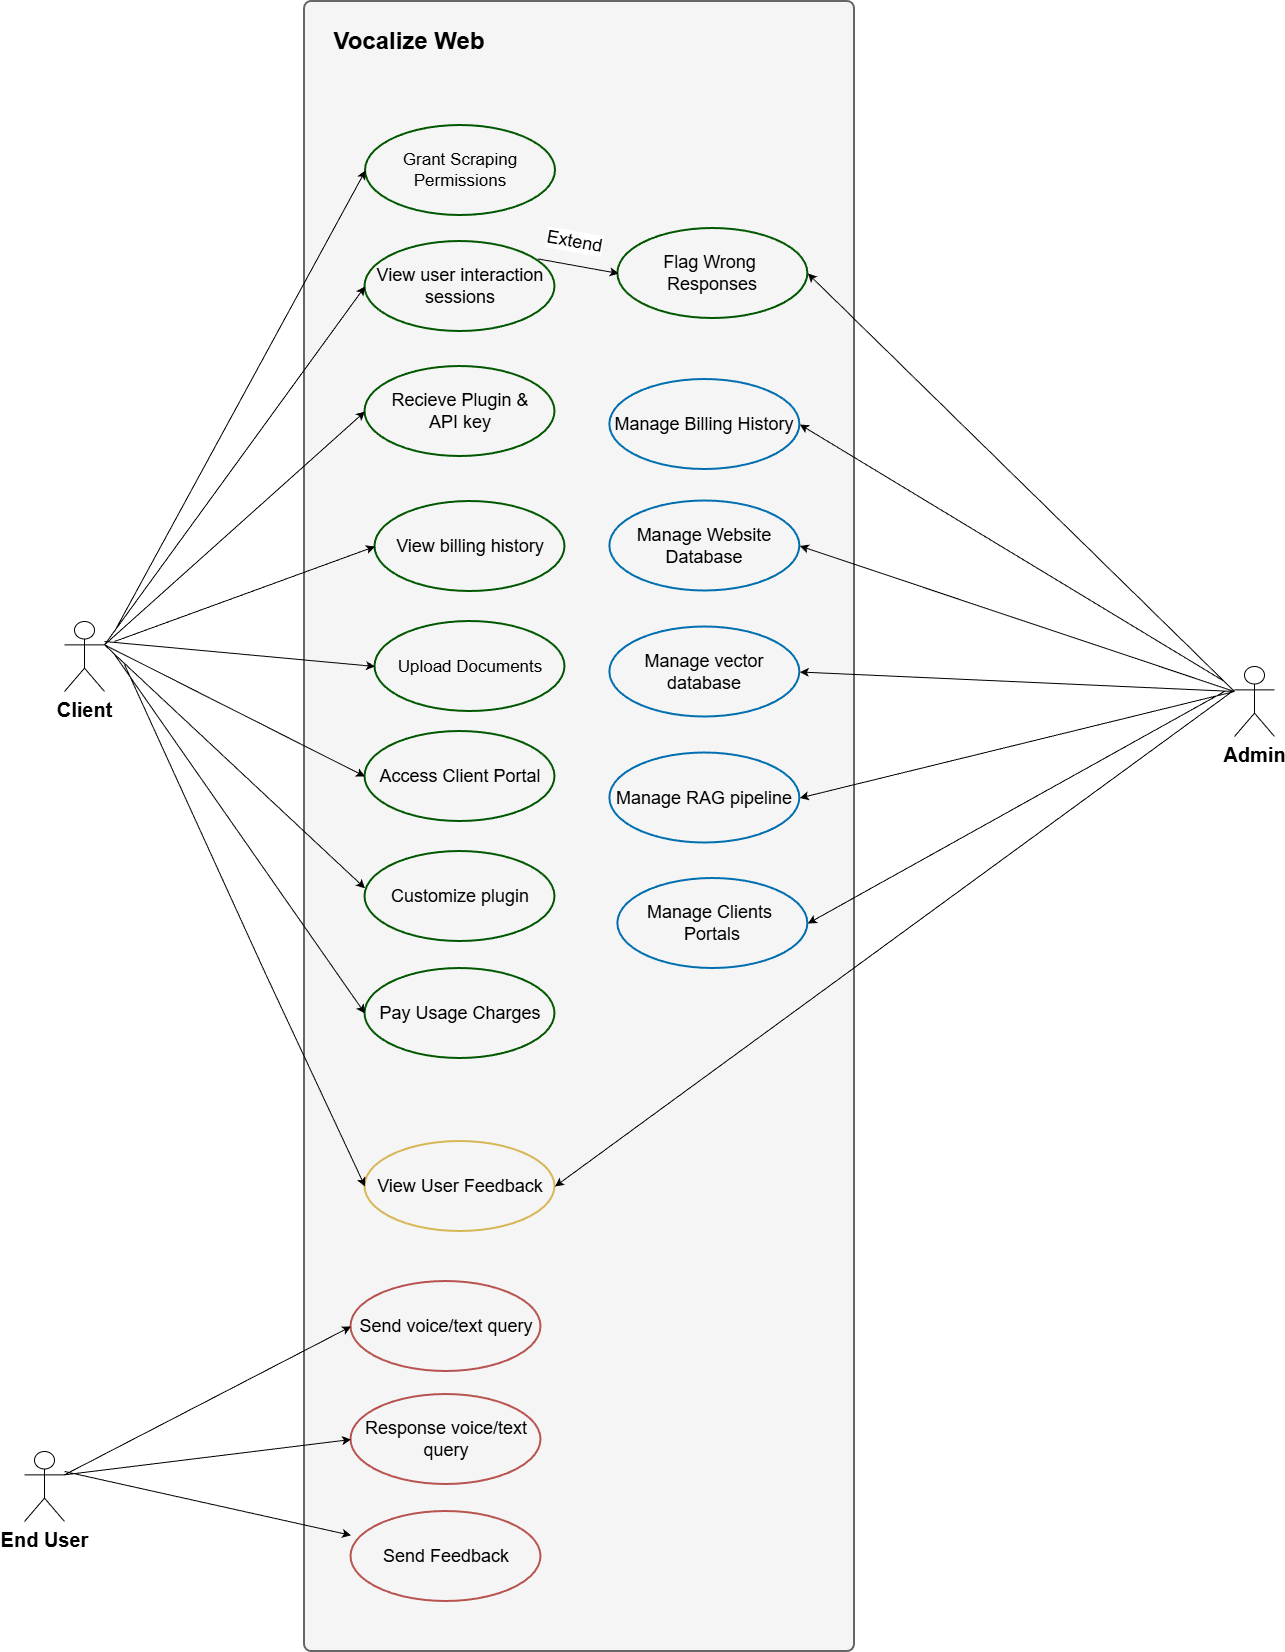
\includegraphics[width=0.95\textwidth]{diagrams/dfd_level_0.png}
    \caption{Level 0 DFD (Context Diagram) - System Boundary View}
    \label{fig:dfd0}
\end{figure}

\subsubsection{Level 1 DFD}

Figure~\ref{fig:dfd1} decomposes the system into major processes: Query Router, Content Ingestion, RAG Pipeline, and Voice Processing. Data stores include Vector DB and SaaS Platform DB.

\begin{figure}[H]
    \centering
    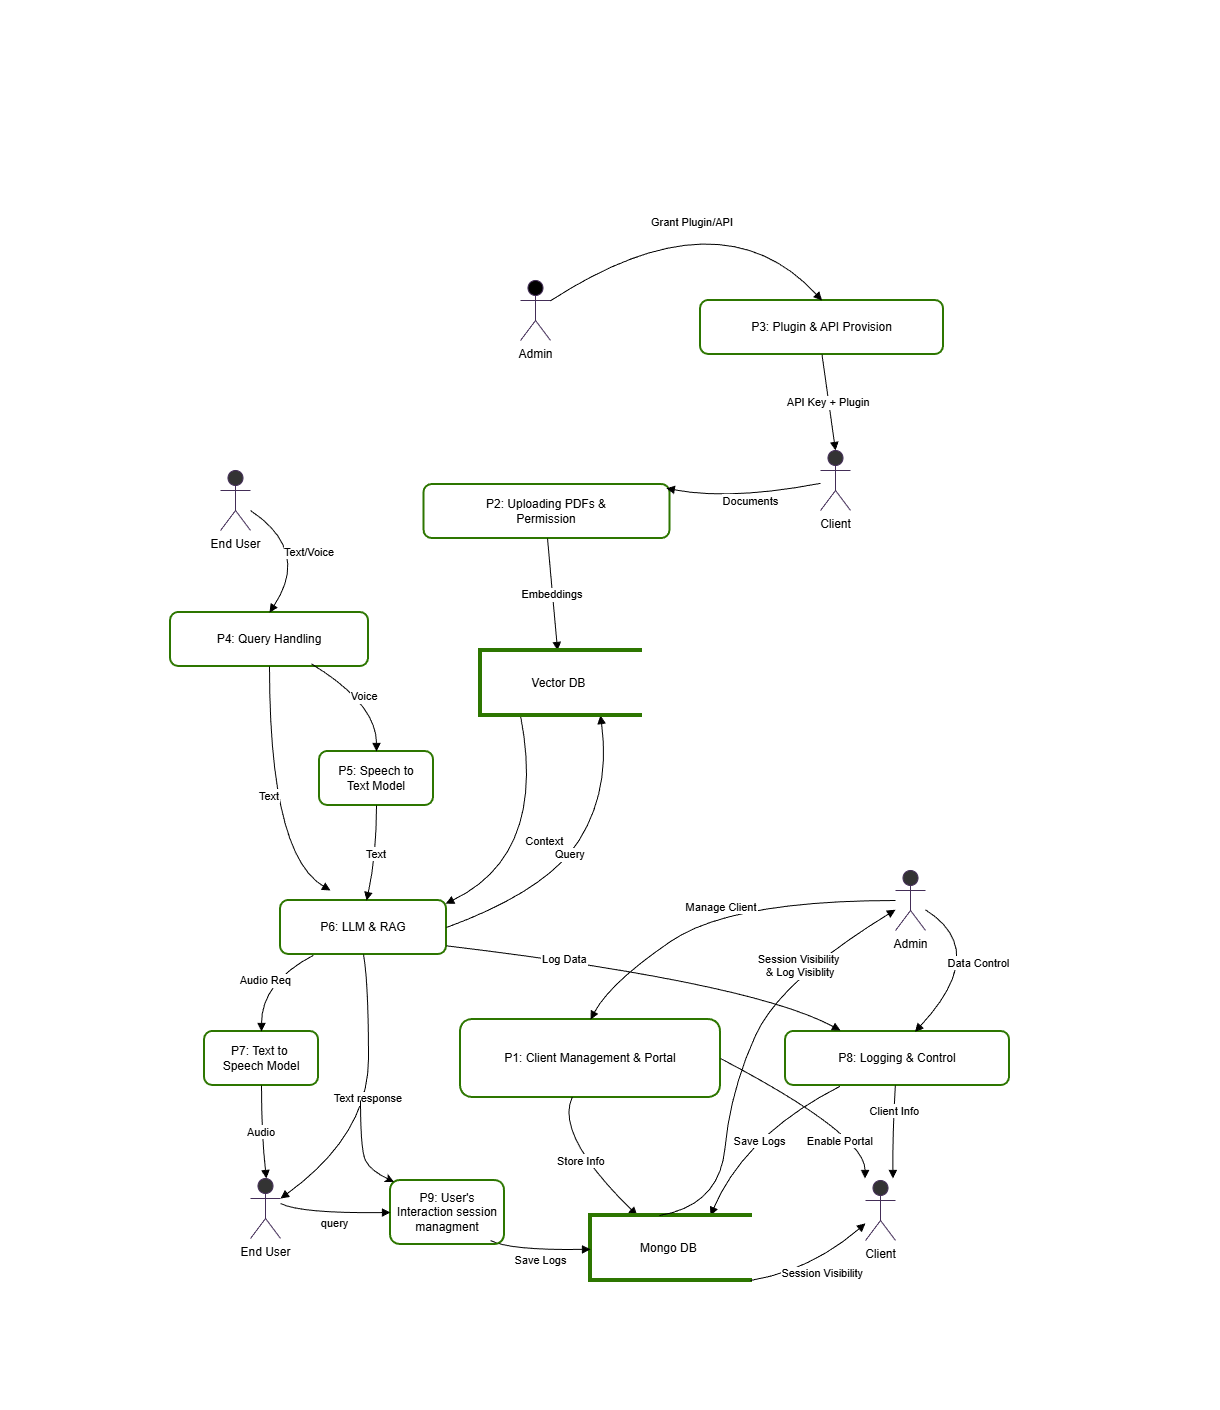
\includegraphics[width=0.85\textwidth]{diagrams/dfd_level1.png}
    \caption{Level 1 DFD - Process Decomposition with Content Types}
    \label{fig:dfd1}
\end{figure}

\subsection{System Architecture Diagram}

Figure~\ref{fig:architecture} presents the high-level system architecture showing the multi-modal frontend, API gateway, processing engines, and multi-database storage layer.

\begin{figure}[H]
    \centering
    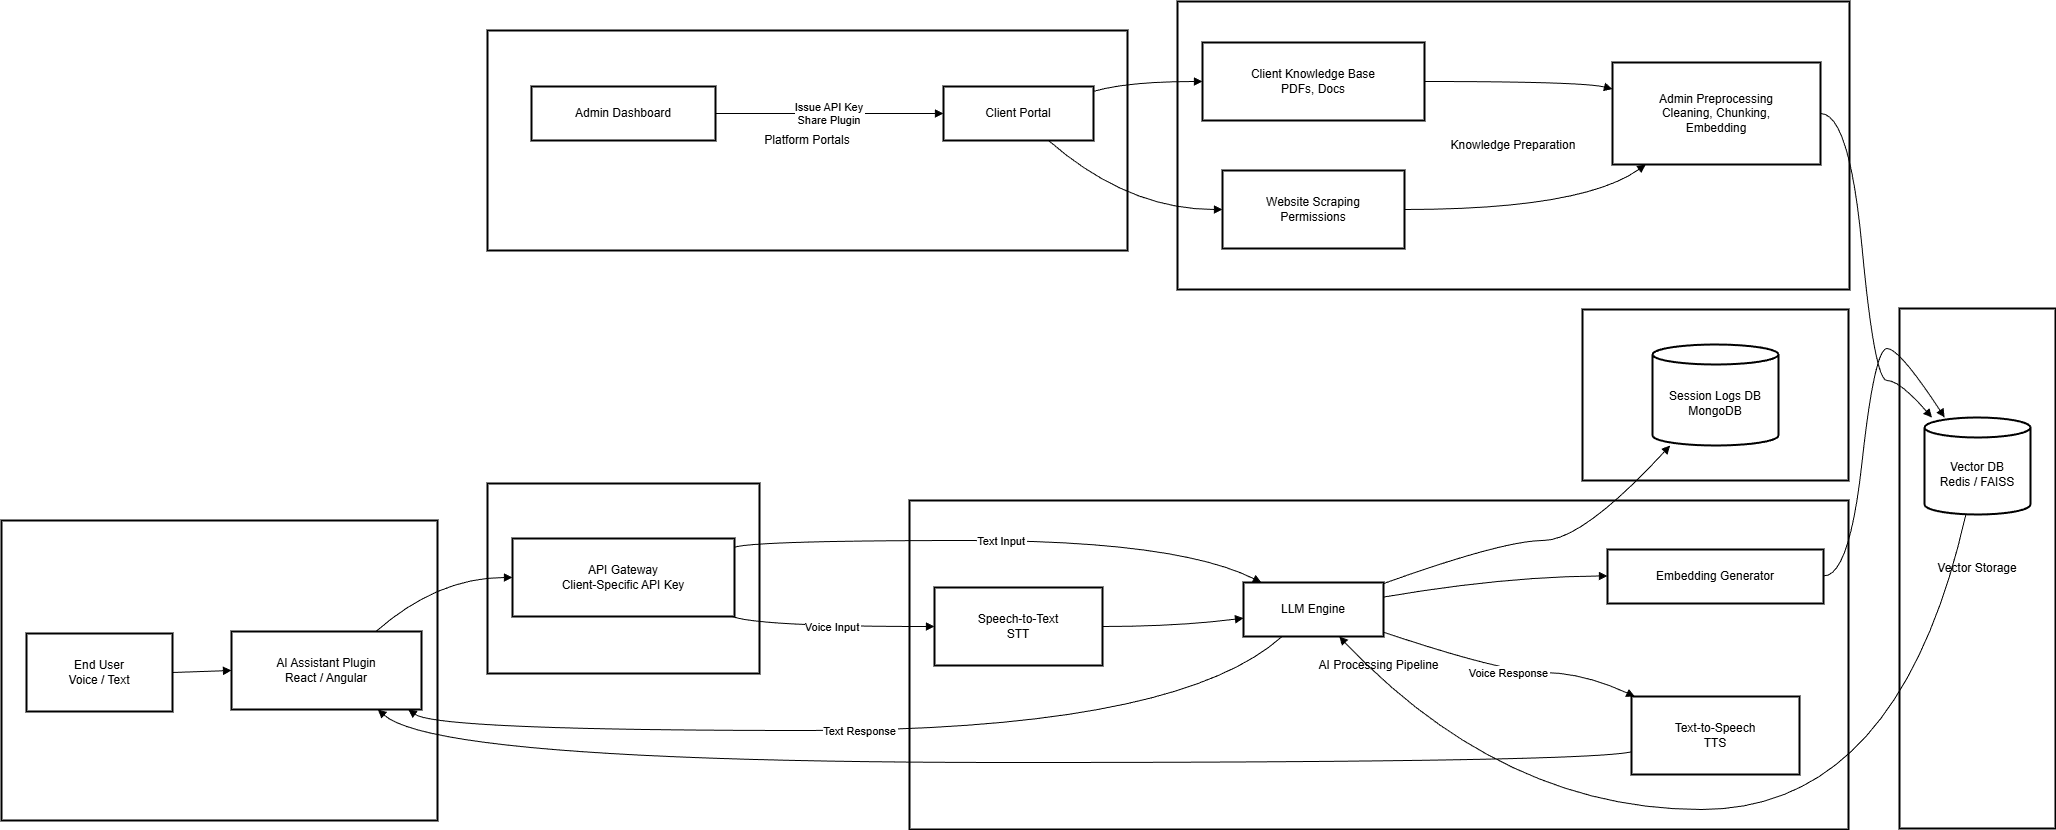
\includegraphics[width=0.95\textwidth]{diagrams/architecture.png}
    \caption{High-Level System Architecture}
    \label{fig:architecture}
\end{figure}

\subsection{Use Case Diagram}

Figure~\ref{fig:usecase} identifies actors (End User, Website Owner, System Admin) and their interactions including multi-modal queries, content management, feature configuration, and DOM synchronization.

\begin{figure}[H]
    \centering
    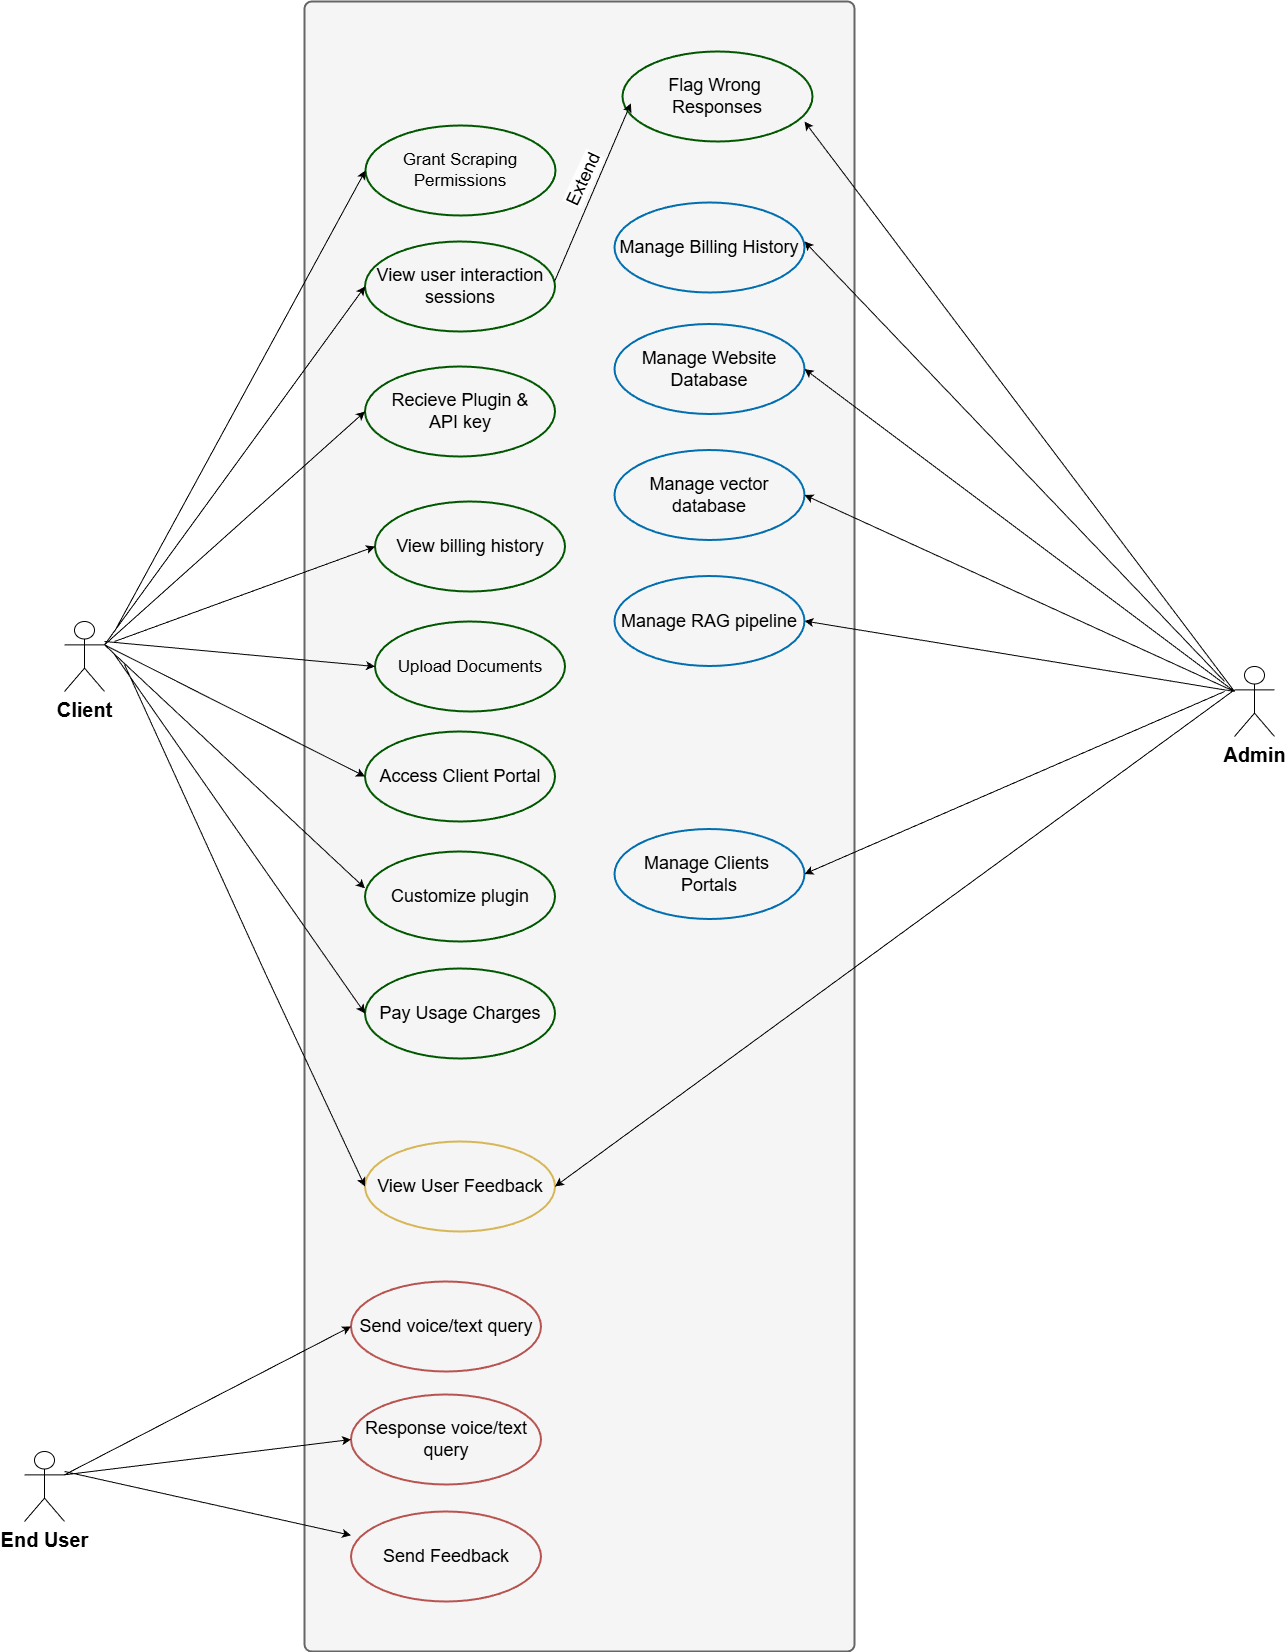
\includegraphics[height=0.75\textheight,keepaspectratio]{diagrams/use_case.png}
    \caption{Use Case Diagram - Actor Interactions}
    \label{fig:usecase}
\end{figure}

\subsection{Entity-Relationship Diagram}

Figure~\ref{fig:erd} models the database schema including Client, KnowledgeBase, ContentItem, Session, Message, and FeatureToggle tables.

\begin{figure}[H]
    \centering
    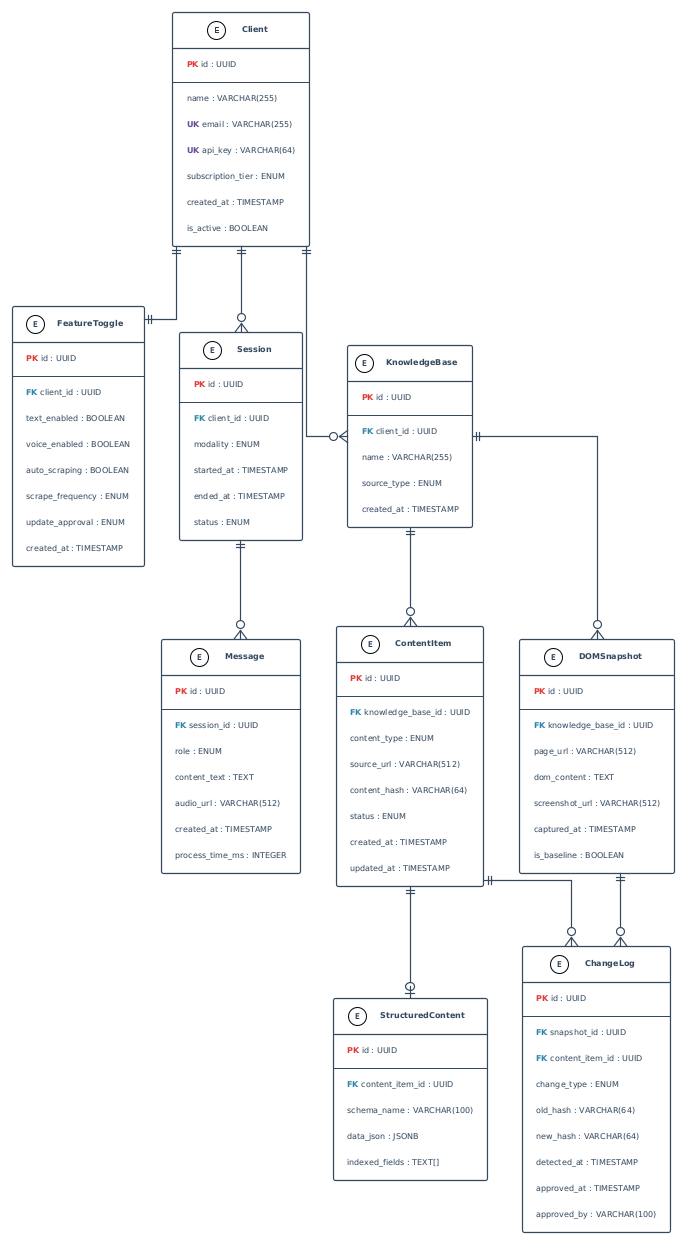
\includegraphics[width=0.85\textwidth]{diagrams/erd.png}
    \caption{Entity-Relationship Diagram - Database Schema}
    \label{fig:erd}
\end{figure}

\subsection{Sequence Diagrams}

\subsubsection{Multi-Modal Query Processing}

Figure~\ref{fig:seq_query} shows the interaction flow for both text and voice queries, including content retrieval from the vector database.

\begin{figure}[H]
    \centering
    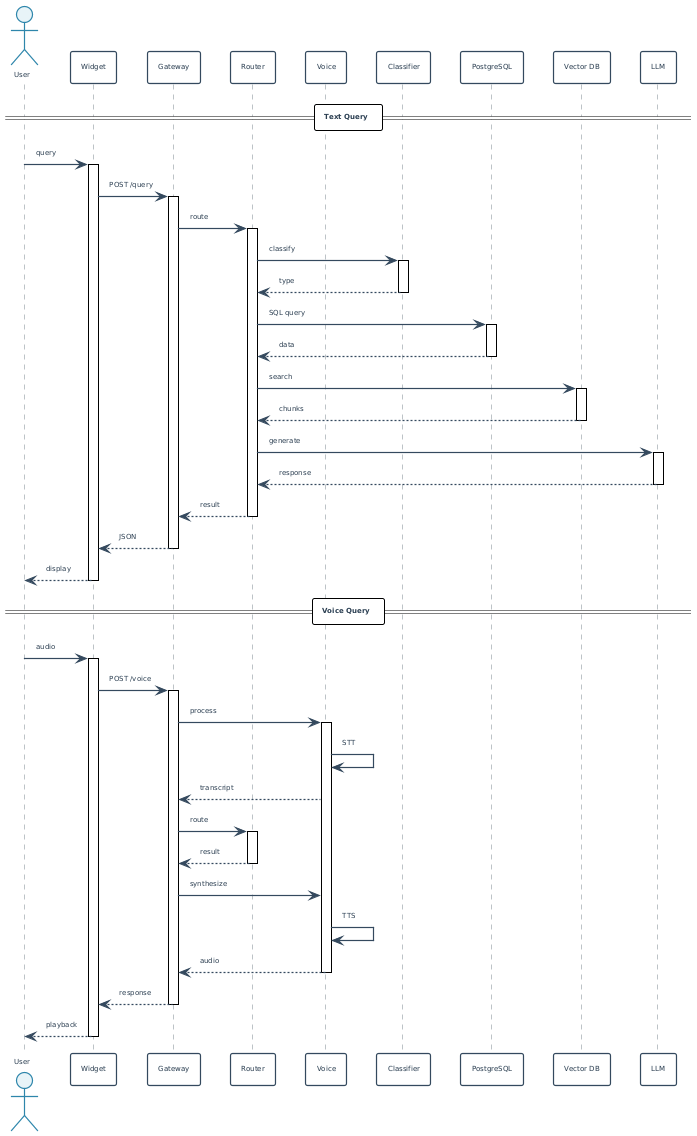
\includegraphics[width=0.95\textwidth]{diagrams/seq_query.png}
    \caption{Sequence Diagram - Multi-Modal Query Processing}
    \label{fig:seq_query}
\end{figure}

\subsubsection{Content Upload and Processing}

Figure~\ref{fig:seq_upload} shows the content upload workflow: document/URL submission, text extraction, chunking, embedding generation, and vector storage.

\begin{figure}[H]
    \centering
    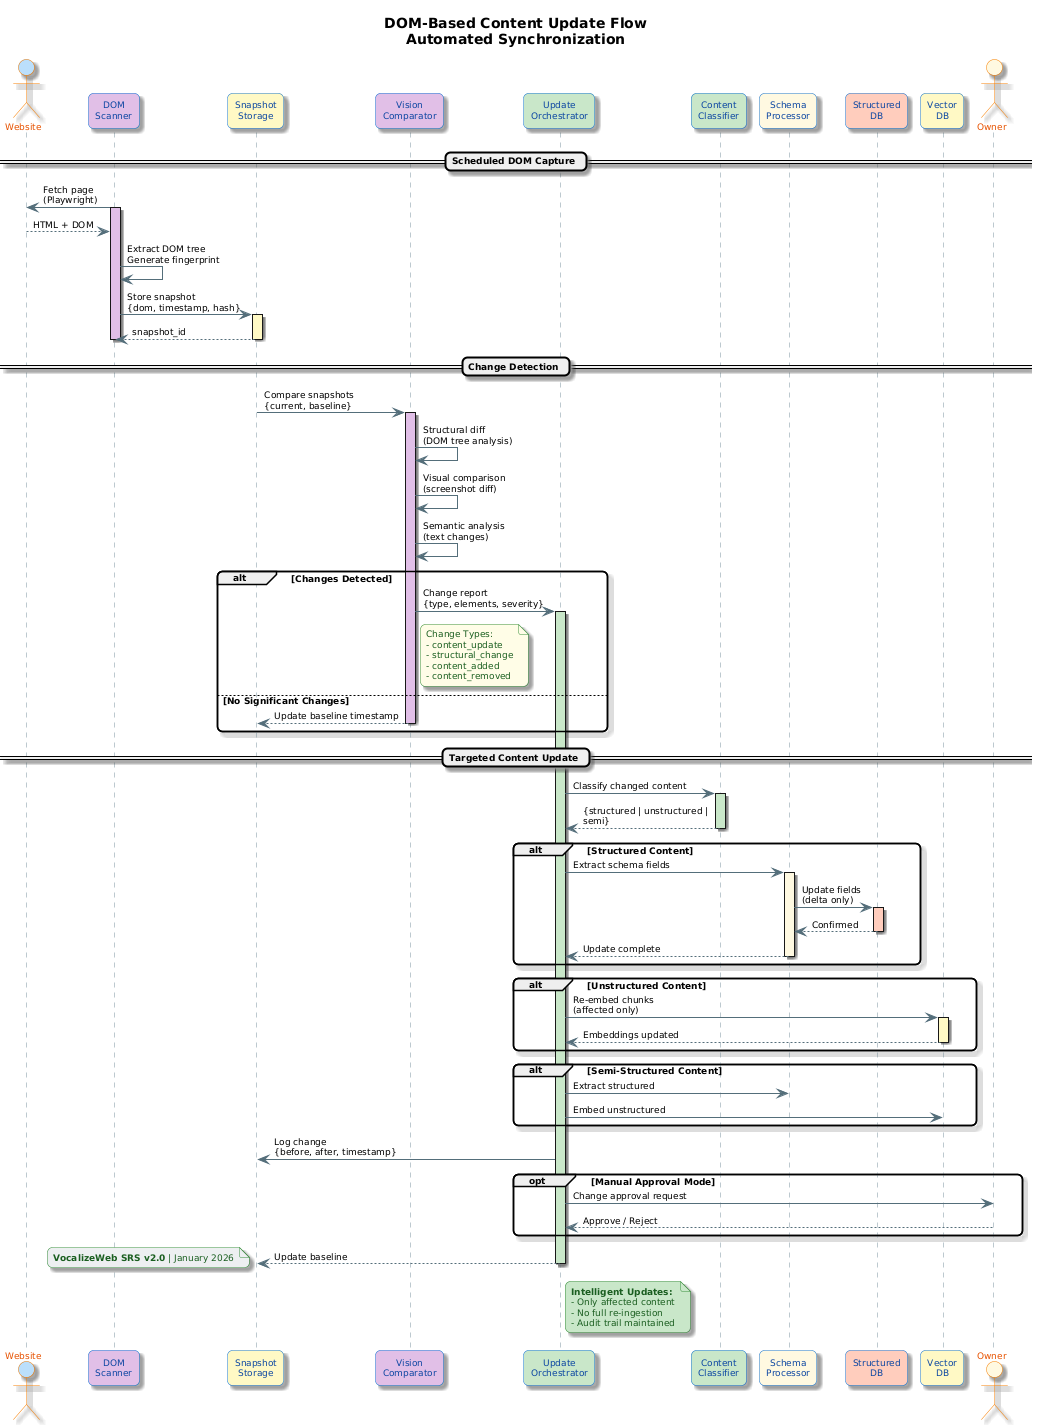
\includegraphics[width=0.95\textwidth]{diagrams/seq_upload.png}
    \caption{Sequence Diagram - Content Upload and Processing Flow}
    \label{fig:seq_upload}
\end{figure}

\section{External Interface Requirements}

\subsection{User Interfaces}

\subsubsection{Multi-Modal Widget}

The primary user interface adapts based on configured modalities:
\begin{itemize}[leftmargin=*]
    \item \textbf{Text Mode:} Floating button expands to chat panel with text input and transcript display
    \item \textbf{Voice Mode:} Floating button activates voice recording with visual states
    \item \textbf{Both Modes:} Combined interface with toggle between text and voice input
\end{itemize}

\subsubsection{Administrative Dashboard}

The dashboard provides:
\begin{itemize}[leftmargin=*]
    \item \textbf{Content Management:} View uploaded content, trigger re-ingestion, manage knowledge base
    \item \textbf{Scraping Configuration:} Configure pages for scraping, view scraping history
    \item \textbf{Feature Toggles:} Enable/disable modalities and auto-update features
    \item \textbf{Analytics:} Usage metrics, query patterns, response quality indicators
\end{itemize}

\subsection{Software Interfaces}

\subsubsection{AI Service Integrations}

\begin{itemize}[leftmargin=*]
    \item \textbf{OpenAI Whisper API:} Audio to text transcription
    \item \textbf{OpenAI Chat Completions:} Response generation with RAG context
    \item \textbf{OpenAI TTS API:} Text to speech synthesis
    \item \textbf{Embedding API:} Vector generation for semantic search
\end{itemize}

\subsubsection{Database Interfaces}

\begin{itemize}[leftmargin=*]
    \item \textbf{PostgreSQL:} Structured content, SaaS platform data via SQLAlchemy ORM
    \item \textbf{Weaviate/Redis:} Vector storage and similarity search via client libraries
\end{itemize}

\section{Constraints and Assumptions}

\subsection{Constraints}

\begin{itemize}[leftmargin=*]
    \item API usage costs for OpenAI services require optimization for profitability
    \item Web scraping frequency limited by target website terms of service
    \item Browser security restrictions limit audio processing capabilities
\end{itemize}

\subsection{Assumptions}

\begin{itemize}[leftmargin=*]
    \item Clients have rights to scrape their own website content
    \item Website structures remain relatively stable between captures
    \item Users have stable internet connectivity for real-time interaction
    \item Target websites do not employ aggressive anti-bot measures
\end{itemize}


% Chapter 4: Remaining Work
% Chapter 4: Remaining Work and Timeline - Updated with Actual Progress
\chapter{Remaining Work}

VocalizeWeb has made significant progress with core functionality now operational. This chapter documents completed work, outlines remaining implementation tasks, and provides project milestones for the enhanced SaaS platform.

\section{Completed Work}

The following core components have been successfully implemented and are fully functional:

\subsection{Speech-to-Speech Pipeline}

\textit{Status:} \textbf{\textcolor{accentgreen}{COMPLETED}}

The complete voice-to-voice interaction pipeline is operational:
\begin{itemize}[leftmargin=*]
    \item Audio capture from browser microphone using Web Audio API
    \item Speech-to-text transcription via OpenAI Whisper Turbo
    \item Natural language processing and response generation
    \item Text-to-speech synthesis using OpenAI TTS
    \item Real-time audio streaming back to user's browser
    \item Voice activity detection and conversation state management
\end{itemize}

\subsection{RAG Pipeline}

\textit{Status:} \textbf{\textcolor{accentgreen}{COMPLETED}}

The Retrieval-Augmented Generation system is fully functional:
\begin{itemize}[leftmargin=*]
    \item Document ingestion and chunking pipeline
    \item Vector embedding generation and storage
    \item Semantic similarity search for context retrieval
    \item LLM integration for response generation with retrieved context
    \item Source citation and grounding in knowledge base
\end{itemize}

\subsection{Embeddable Widget Plugin}

\textit{Status:} \textbf{\textcolor{accentgreen}{COMPLETED}}

The plug-and-play widget for website integration is built:
\begin{itemize}[leftmargin=*]
    \item Single JavaScript snippet deployment
    \item Floating chat/voice button interface
    \item Responsive design for mobile and desktop
    \item Customizable styling and positioning
    \item Session management and conversation persistence
\end{itemize}

\section{Remaining Work}

\subsection{Phase 1: SaaS Platform Enhancement}

Core platform features that enhance the multi-tenant capabilities.

\vspace{0.3cm}

\textbf{Task 1.1: Enhanced Content Management}

\textit{Status:} Not Started

\textit{Description:} Develop comprehensive content management interface allowing clients to upload documents, configure scraping, and manage knowledge base updates.

\textit{Dependencies:} None (can start immediately)

\vspace{0.3cm}

\textbf{Task 1.2: Advanced Analytics Dashboard}

\textit{Status:} Not Started

\textit{Description:} Build React-based analytics dashboard showing usage metrics, query patterns, response quality, and user engagement statistics.

\textit{Dependencies:} Backend API endpoints

\vspace{0.3cm}

\textbf{Task 1.3: Feature Toggle System Enhancement}

\textit{Status:} Not Started

\textit{Description:} Implement granular per-client feature configuration for modalities, content sources, and platform capabilities.

\textit{Dependencies:} Database schema updates

\subsection{Phase 2: Production Deployment}

\textbf{Task 2.1: Infrastructure Setup}

\textit{Status:} Not Started

\textit{Description:} Set up production servers, database clusters, load balancing, and monitoring infrastructure.

\textit{Dependencies:} Server provisioning

\vspace{0.3cm}

\textbf{Task 2.2: Security Hardening}

\textit{Status:} Not Started

\textit{Description:} Implement rate limiting, API key rotation, input validation, and security audits.

\textit{Dependencies:} Production infrastructure

\vspace{0.3cm}

\textbf{Task 2.3: Performance Optimization}

\textit{Status:} Not Started

\textit{Description:} Optimize query processing, caching strategies, and database indexing for production workloads.

\textit{Dependencies:} Load testing results

\section{Milestones}

\begin{table}[H]
\centering
\caption{\textit{Project Milestones}}
\begin{tabularx}{\textwidth}{|l|X|l|}
\hline
\textbf{Milestone} & \textbf{Description} & \textbf{Status} \\
\hline
M1: Voice Pipeline & Speech-to-speech interaction working & \textcolor{accentgreen}{\textbf{Done}} \\
\hline
M2: RAG System & Retrieval-augmented generation operational & \textcolor{accentgreen}{\textbf{Done}} \\
\hline
M3: Widget Plugin & Embeddable website plugin deployed & \textcolor{accentgreen}{\textbf{Done}} \\
\hline

M4: Analytics Dashboard & Usage analytics and monitoring deployed & Pending \\
\hline
\end{tabularx}
\end{table}

\section{Progress Summary}

\begin{table}[H]
\centering
\caption{\textit{Overall Project Progress}}
\begin{tabularx}{\textwidth}{|X|c|c|}
\hline
\textbf{Component} & \textbf{Status} & \textbf{Completion} \\
\hline
Speech-to-Speech Pipeline & \textcolor{accentgreen}{\textbf{Completed}} & 100\% \\
\hline
RAG Pipeline & \textcolor{accentgreen}{\textbf{Completed}} & 100\% \\
\hline
Embeddable Widget & \textcolor{accentgreen}{\textbf{Completed}} & 100\% \\
\hline
SaaS Platform Features & Not Started & 0\% \\ \\
\hline
\multicolumn{2}{|r|}{\textbf{Overall Project Progress}} & \textbf{60\%} \\
\hline
\end{tabularx}
\end{table}

\section{Risk Management}

\subsection{Technical Risks}

\begin{itemize}[leftmargin=*]
    \item \textbf{Web Scraping Restrictions:} Target websites may block automated access. \textit{Mitigation:} Respectful rate limiting, user-agent configuration, client-owned content only.
    \item \textbf{API Cost Management:} OpenAI API usage costs require careful monitoring. \textit{Mitigation:} Caching strategies, prompt optimization, usage quotas.
\end{itemize}

\subsection{Schedule Risks}

\begin{itemize}[leftmargin=*]
    \item \textbf{Platform Complexity:} Full-featured SaaS platform requires significant development effort. \textit{Mitigation:} MVP-first approach, iterative feature addition, code reusability.
    \item \textbf{Production Scaling:} Multi-tenant architecture requires careful resource management. \textit{Mitigation:} Load testing, horizontal scaling design, performance benchmarks.
\end{itemize}

\section{Future Enhancements}

Beyond the current development roadmap, the following advanced features are planned for future releases to further differentiate VocalizeWeb in the market:

\subsection{Phase 3: DOM-Based Auto-Update System (Future)}

This advanced feature will automate content synchronization and eliminate manual knowledge base updates.

\vspace{0.3cm}

\textbf{Task 3.1: DOM Snapshot Engine}

\textit{Status:} Planned for Future Release

\textit{Description:} Develop headless browser automation (Playwright) to capture DOM snapshots of configured web pages at scheduled intervals. Store snapshots with timestamps and content fingerprints for change comparison.

\textit{Dependencies:} Stable SaaS platform deployment

\vspace{0.3cm}

\textbf{Task 3.2: Vision-Based Change Detection}

\textit{Status:} Planned for Future Release

\textit{Description:} Integrate open-source computer vision models to perform structural and visual comparison of DOM snapshots. Classify changes as content updates, structural changes, or style-only modifications.

\textit{Dependencies:} DOM Snapshot Engine, GPU infrastructure

\vspace{0.3cm}

\textbf{Task 3.3: Intelligent Content Classification}

\textit{Status:} Planned for Future Release

\textit{Description:} Implement automatic categorization of website content as structured (e.g., product catalogs, faculty directories), unstructured (e.g., blogs, FAQs), or semi-structured (e.g., mixed HTML sections) for optimized storage and retrieval.

\textit{Dependencies:} Machine learning model training

\vspace{0.3cm}

\textbf{Task 3.4: Targeted Update Orchestrator}

\textit{Status:} Planned for Future Release

\textit{Description:} Build intelligent update logic that triggers re-processing of only affected content chunks when changes are detected, avoiding expensive full knowledge base rebuilds.

\textit{Dependencies:} Change detection, content classification

\vspace{0.3cm}

\textbf{Expected Benefits:}
\begin{itemize}[leftmargin=*]
    \item \textbf{Zero Manual Intervention:} Assistant knowledge stays current automatically
    \item \textbf{Cost Efficiency:} Incremental updates reduce computational overhead
    \item \textbf{Competitive Advantage:} No competitor currently offers automated change detection
    \item \textbf{Trust and Accuracy:} Users always receive up-to-date information
\end{itemize}



% References
% References - Professional Bibliography
\chapter*{References}
\addcontentsline{toc}{chapter}{References}

\vspace{-0.5cm}

\begin{infobox}[Citation Standards]
All references in this document follow IEEE citation format as per IEEE Reference Guide. References are numbered in the order of their first appearance and cited using bracketed numerals.
\end{infobox}

\vspace{0.5cm}

\begin{thebibliography}{99}

% Standards
\bibitem{ieee29148}
IEEE, ``ISO/IEC/IEEE 29148:2018 --- Systems and software engineering --- Life cycle processes --- Requirements engineering,'' \textit{IEEE Standards Association}, 2018. [Online]. Available: \url{https://standards.ieee.org/standard/29148-2018.html}

% Speech Recognition
\bibitem{whisper}
A. Radford, J. W. Kim, T. Xu, G. Brockman, C. McLeavey, and I. Sutskever, ``Robust Speech Recognition via Large-Scale Weak Supervision,'' \textit{arXiv preprint arXiv:2212.04356}, Dec. 2022. [Online]. Available: \url{https://arxiv.org/abs/2212.04356}

% Large Language Models
\bibitem{gpt4}
OpenAI, ``GPT-4 Technical Report,'' \textit{arXiv preprint arXiv:2303.08774}, Mar. 2023. [Online]. Available: \url{https://arxiv.org/abs/2303.08774}

% RAG Architecture
\bibitem{rag}
P. Lewis, E. Perez, A. Piktus, F. Petroni, V. Karpukhin, N. Goyal, \textit{et al.}, ``Retrieval-Augmented Generation for Knowledge-Intensive NLP Tasks,'' in \textit{Advances in Neural Information Processing Systems (NeurIPS)}, vol. 33, pp. 9459--9474, 2020.

% Vector Databases
\bibitem{weaviate}
SeMI Technologies, ``Weaviate: Open-source vector database,'' 2024. [Online]. Available: \url{https://weaviate.io}. [Accessed: Jan. 2026]

% Competitor Platforms
\bibitem{webvoice}
Webvoice AI, ``Webvoice AI --- The AI Voice Agent for Your Website,'' 2024. [Online]. Available: \url{https://webvoice.chat}. [Accessed: Jan. 2026]

\bibitem{chatbotsforwebsites}
ChatbotsForWebsites.ai, ``AI Frontline Operations Platform (Chat + Phone),'' 2024. [Online]. Available: \url{https://chatbotsforwebsites.ai}. [Accessed: Jan. 2026]

\bibitem{speak2web}
Speak2Web, ``Speak2Web --- Voice-First Website Interaction,'' 2024. [Online]. Available: \url{https://speak2web.ai}. [Accessed: Jan. 2026]

\bibitem{voicemysite}
VoiceMySite, ``VoiceMySite --- \#1 Voice Chatbot Platform for Websites | AI Voice Agents,'' 2024. [Online]. Available: \url{https://www.voicemysite.com}. [Accessed: Jan. 2026]

\bibitem{aiconnect}
AIConnect.chat, ``AIConnect.chat --- Turn your website into a real-time voice conversation,'' 2024. [Online]. Available: \url{https://www.aiconnect.chat}. [Accessed: Jan. 2026]

\bibitem{realvoice}
RealVoice AI, ``Give Your Site a Voice | AI Voice Widget for Websites,'' 2024. [Online]. Available: \url{https://www.realvoice.ai}. [Accessed: Jan. 2026]

\end{thebibliography}

\vspace{1cm}

\noindent\textcolor{gray}{\rule{\textwidth}{0.5pt}}

\vspace{0.5cm}

\noindent\textit{\small Help has been taken from the above resources in the preparation of this document. We acknowledge the authors and organizations for making their research and documentation publicly available.}


% Appendices
% Appendices - Revised for Intelligent Content Management Platform
\appendix
\addcontentsline{toc}{chapter}{Appendices}

\chapter{API Specification Examples}

\section{Query Endpoints}

\subsection{Text Query}

\textbf{Endpoint:} POST /api/v1/query

\textbf{Headers:}
\begin{lstlisting}
Authorization: Bearer <API_KEY>
Content-Type: application/json
\end{lstlisting}

\textbf{Request Body:}
\begin{lstlisting}
{
  "session_id": "sess_7f8a9b0c",
  "query": "What are your shipping options?",
  "modality": "text"
}
\end{lstlisting}

\textbf{Response:}
\begin{lstlisting}
{
  "message_id": "msg_1a2b3c4d",
  "response": "We offer standard, express...",
  "sources": [
    {"type": "structured", "ref": "shipping_policies"},
    {"type": "unstructured", "ref": "faq_chunk_42"}
  ],
  "processing_time_ms": 2340
}
\end{lstlisting}

\subsection{Voice Query}

\textbf{Endpoint:} POST /api/v1/voice-query

\textbf{Request Body:} multipart/form-data with audio file
\begin{lstlisting}
{
  "session_id": "sess_7f8a9b0c",
  "audio": <binary>,
  "format": "wav"
}
\end{lstlisting}

\textbf{Response:}
\begin{lstlisting}
{
  "message_id": "msg_1a2b3c4d",
  "transcript": "What are your shipping options?",
  "response_text": "We offer standard, express...",
  "response_audio_url": "https://cdn.vocalizeweb.com/...",
  "processing_time_ms": 4320
}
\end{lstlisting}

\section{Content Management Endpoints}

\subsection{Configure Scraping}

\textbf{Endpoint:} POST /api/v1/scraping/configure

\begin{lstlisting}
{
  "pages": [
    {
      "url": "https://example.com/products",
      "content_type": "structured",
      "schema": "product_catalog"
    },
    {
      "url": "https://example.com/faq",
      "content_type": "unstructured"
    }
  ],
  "frequency": "daily"
}
\end{lstlisting}

\subsection{Get DOM Changes}

\textbf{Endpoint:} GET /api/v1/changes?status=pending

\begin{lstlisting}
{
  "changes": [
    {
      "id": "chg_abc123",
      "page_url": "https://example.com/products",
      "change_type": "content_update",
      "detected_at": "2026-01-13T08:00:00Z",
      "affected_items": 3,
      "status": "pending_approval"
    }
  ]
}
\end{lstlisting}

\chapter{Content Schema Examples}

\section{Product Catalog Schema}

\begin{lstlisting}
{
  "schema_name": "product_catalog",
  "fields": [
    {"name": "product_id", "type": "string", "required": true},
    {"name": "name", "type": "string", "required": true},
    {"name": "price", "type": "decimal", "required": true},
    {"name": "currency", "type": "string", "default": "USD"},
    {"name": "availability", "type": "enum", 
     "values": ["in_stock", "out_of_stock", "preorder"]},
    {"name": "description", "type": "text", "embed": true},
    {"name": "category", "type": "string", "indexed": true}
  ],
  "dom_selectors": {
    "container": ".product-card",
    "product_id": "[data-product-id]",
    "name": ".product-title",
    "price": ".price-current",
    "availability": ".stock-status"
  }
}
\end{lstlisting}

\section{Faculty Directory Schema}

\begin{lstlisting}
{
  "schema_name": "faculty_directory",
  "fields": [
    {"name": "name", "type": "string", "required": true},
    {"name": "department", "type": "string", "indexed": true},
    {"name": "designation", "type": "string"},
    {"name": "email", "type": "email"},
    {"name": "phone", "type": "string"},
    {"name": "office", "type": "string"},
    {"name": "bio", "type": "text", "embed": true},
    {"name": "courses", "type": "array[string]"}
  ]
}
\end{lstlisting}

\chapter{Feature Toggle Configuration}

\section{Toggle Options}

\begin{lstlisting}
{
  "client_id": "client_abc123",
  "toggles": {
    "interaction_mode": "both",  // text | voice | both
    "auto_scraping": true,
    "scrape_frequency": "daily", // hourly | daily | weekly | manual
    "update_approval": "manual", // manual | automatic
    "conversation_storage": "full", // full | summary | none
    "analytics_access": "admin"  // admin | shared | none
  }
}
\end{lstlisting}

\chapter{Server Specifications}

\section{Production Requirements}

\begin{table}[H]
\centering
\begin{tabular}{|l|l|}
\hline
\textbf{Component} & \textbf{Specification} \\
\hline
Application Servers & 4 cores, 16 GB RAM, Python 3.10+ \\
\hline
PostgreSQL Database & 4 cores, 32 GB RAM, 500 GB SSD \\
\hline
Vector Database & Weaviate cluster or Redis with RediSearch \\
\hline
DOM Scanner Workers & 2 cores, 8 GB RAM per worker (Playwright) \\
\hline
Vision Model Inference & GPU recommended (NVIDIA T4 or better) \\
\hline
Network & 1 Gbps, low latency to AI service providers \\
\hline
\end{tabular}
\end{table}

\chapter{Glossary}

\begin{table}[H]
\centering
\begin{tabular}{|l|p{10cm}|}
\hline
\textbf{Term} & \textbf{Definition} \\
\hline
Content Type & Classification of content as structured, unstructured, or semi-structured \\
\hline
DOM Snapshot & Stored representation of a webpage's Document Object Model at a point in time \\
\hline
Feature Toggle & Configuration flag controlling enabled capabilities per client \\
\hline
Vision Comparator & AI model comparing DOM snapshots to detect changes \\
\hline
Schema-Driven Ingestion & Extracting content according to predefined field definitions \\
\hline
Targeted Update & Updating only content affected by detected changes \\
\hline
Multi-Modal & Supporting multiple interaction modalities (text and voice) \\
\hline
\end{tabular}
\end{table}


\end{document}
